\selectlanguage{english}%

\section{Cartesian Lattice \protect \\
Q-space Reconstructions\label{sec:Cartesian-Lattice-Q-space}}


\subsection{Overview}

Between one to two thirds of imaging voxels in the human brain's white
matter are thought to contain multiple fibre bundle crossings~\cite{Behrens2007NeuroImage},
in which case the Diffusion Tensor model proposed by Basser et al.~\cite{Basser1994}
breaks down. High Angular Resolution Diffusion Imaging (HARDI) methods
\cite{Tuch2002} such as Diffusion Spectrum Imaging (DSI)~\cite{callaghan1988nmr},
\cite{wedeen2005mapping} or Higher Order Tensors~\cite{ozarslan2003generalized},
\cite{barmpoutis2009regularized} and many more reconstruction methods
have been proposed to overcome the limitations of the Diffusion Tensor.
These methods can be divided into those which need specific acquisition
parametrizations, and those which can be used independently of q-space
structure. For instance, for Q-ball Imaging~\cite{Tuch2004} sampling
needs to be on one or more spherical grids, and in Generalized Q-sampling
Imaging (GQI)~\cite{Yeh2010}, requires sampling on a Cartesian grid;
by contrast DTI can be used independently of q-space structure. A
further division considers the level of model assumptions for the
diffusion process. Although all methods have some underlying assumptions
we generally separate them in model-based and model-free. Model-based
methods like the Single Tensor or Multi Tensor require a number of
parameters to be fitted. By contrast, in model-free methods fitting
is not necessary and the directionality of the underlying tissue can
be approximated by some re-parametrization or re-transformation of
the signal. The latter is usually more efficient than fitting models
with many parameters which typically call for iterative methods.

This chapter presents, evaluates and compares different model-free
methods for the reconstruction of orientation distribution functions
using diffusion MRI data sampled on a Cartesian lattice in q-space.
This non-parametric nature of the algorithms described here allows
for the identification of multiple fibre crossings. In addition, a
new method is presented named Diffusion Nabla Imaging (DNI) and a
family of methods is defined called the Equatorial Inversion Transform
(EIT). The EIT is a new way to represent and reconstruct the diffusion
signal. Our results show that EIT can perform better or as well as
the current state-of-the art methods i.e. DSI and GQI.


\subsection{Theory}

We start from the classical formulation shown in Eq.~\ref{eq:kq}
of joint k-space and q-space imaging described in Callaghan~\cite{Callaghan1991OUP},
\cite{callaghan1988nmr} using the narrow pulse gradient spin echo
(PGSE) sequence of Tanner and Stejskal \begin{eqnarray}
RF(\mathbf{k},\mathbf{q}) & = & \int\rho(\mathbf{v})\exp(i2\pi\mathbf{k}\cdot\mathbf{v})\int P_{\Delta}(\mathbf{v},\mathbf{r})\exp(i2\pi\mathbf{q}\cdot\mathbf{r})\, d\mathbf{r\,}d\mathbf{v}\label{eq:kq}\end{eqnarray}


\noindent Here $RF$ represents the complex RF signal measured at
spatial wave number $\mathbf{k}$ and magnetic gradient wave number
$\mathbf{q}$, $\rho$ is the local spin density (number of protons
per unit volume contributing to the RF signal), $\Delta$ is the time
between diffusion gradients, $P_{\Delta}$ is the average diffusion
propagator (transition probability distribution), \textbf{$\mathbf{v}$}
is the voxel coordinate, and $\mathbf{r}$ is the diffusion displacement. 

The k-space reconstruction gives us diffusion weighted image data
$S$ which reveal the average propagator $P_{\Delta}$ of each voxel
\begin{eqnarray}
S(\mathbf{v},\mathbf{q}) & = & \int\rho(\mathbf{v})P_{\Delta}(\mathbf{v},\mathbf{r})\exp(i2\pi\mathbf{q}\cdot\mathbf{r})d\mathbf{r}\label{eq:W}\end{eqnarray}


For the rest of the chapter we consider each voxel independently and
assume intra-voxel spatial homogeneity so we can drop explicit reference
to $\mathbf{v}$ and $\Delta$. We note in passing that the shape
of $P_{\Delta}$ and hence of the ODF may change with different values
of $\Delta$. We will not pursue this matter further here. We can
also replace the spin density \foreignlanguage{british}{$\rho(\mathbf{v})$}
with $S_{0}$ i.e. the measured signal without diffusion weighting
$\mathbf{q}=\mathbf{0}$. Therefore we can write\begin{eqnarray}
S(\mathbf{q}) & = & S_{0}\int P(\mathbf{r})\exp(i2\pi\mathbf{q}\cdot\mathbf{r})d\mathbf{r}\label{eq:S}\end{eqnarray}


By applying the 3D Fourier transform in Eq.~\ref{eq:S} we can reconstruct
the average propagator also known as the diffusion spectrum \cite{Wedeen}
or diffusion propagator\begin{eqnarray}
P(\mathbf{r}) & = & S_{0}^{-1}\int S(\mathbf{q})\exp(-i2\pi\mathbf{q}\cdot\mathbf{r})d\mathbf{r}\label{eq:P}\end{eqnarray}


\noindent It was shown by Wedeen et al. \cite{Wedeen} that the dMRI
signal is positive for any type of spin motion without net flux (i.e.~spin
displacements due to thermal molecular agitation) or other random
fluxes such as intravoxel incoherent motion. Under this assumption
we can replace the complex signal $S$ with its modulus $|S|$ in
Eq.~\ref{eq:P} \begin{eqnarray}
P(\mathbf{r}) & = & S_{0}^{-1}\int|S(\mathbf{q})|\exp(-i2\pi\mathbf{q}\cdot\mathbf{r})d\mathbf{r}\label{eq:P_modulus}\end{eqnarray}


The modulus of the signal coincides with the output of the standard
MRI scanners as dMRI and that simplifies the acquisition procedure.
It represents the density of the average relative spin displacement
in a voxel. In other words, $P(\mathbf{r})\, d\mathbf{r}$ is a measure
of the probability that a spin in a chosen voxel , during the experimental
mixing time $\Delta$, would make a vector displacement $\mathbf{r}$.
We can visualize the propagator for every voxel as a 3D density volume
(see Fig.~\ref{Flo:ODF}).

In the classical Q-ball acquisition, at each location, diffusion-weighted
images are acquired for $N=515$ or fewer values of q-encoding, comprising
in q-space the points of a cubic lattice within the sphere of five
lattice units in radius. Therefore,\begin{eqnarray}
\mathbf{q} & = & \alpha\mathbf{q}_{x}+\beta\mathbf{q}_{y}+\gamma\mathbf{q}_{z}\label{eq:q_lattice}\end{eqnarray}


\noindent with $\alpha,\beta,\gamma\in\mathbb{Z}^{+}$ and $(\alpha^{2}+\beta^{2}+\gamma^{2})^{1/2}\leq5$.
The signal is premultiplied by a Hanning window before Fourier transform
in order to ensure a smooth attenuation of the signal at high $q$
values. Often, to obtain data for the complete grid of $515$ q-vectors
(which also means that we need to collect $515$ diffusion weighted
volumes), the overall acquisition time would be too long and a smaller
number of unique q-vectors are employed for just a single hemisphere
usually between $101$ to $257$ points~\cite{Kuo}. This is valid
because the underlying self-diffusion process is symmetric and so
the signal is symmetric, therefore the vectors can be mapped on the
other hemisphere to create the full q-space. 

Since we are mainly interested in the angular structure of the underlying
tissue, we further simplify the data by taking the weighted radial
summation of $P(\mathbf{r})$\foreignlanguage{british}{\begin{equation}
\psi_{DSI}(\hat{\mathbf{u}})=\int_{0}^{\infty}P(r\hat{\mathbf{u}})r^{2}dr\label{eq:ODF_DSI}\end{equation}
}

\noindent This defines the \foreignlanguage{british}{orientation
density function (ODF) for DSI which measures the quantity of diffusion
in the direction of the unit vector $\mathbf{\hat{u}}$ where $\mathbf{r=}r\hat{\mathbf{u}}$.}

\selectlanguage{british}%
Note at this point that in order to find the ODF we have to first
create the diffusion propagator by \foreignlanguage{english}{applying}
the Fourier transform on the lattice. \foreignlanguage{english}{Yeh
et al.~\cite{Yeh2010} proposed a direct way to calculate a slightly
different ODF using the Cosine transform.}

\selectlanguage{english}%
In order to represent the average propagator in the scale of spin
quantity Yeh et al.~\cite{Yeh2010} introduced the \emph{spin density
function }$Q$ which is estimated by scaling the average propagator
$P_{\Delta}$ with the spin density $\rho$, i.e. $Q(\mathbf{r})=\rho P(\mathbf{r})=S_{0}P(\mathbf{r})$.
From Eq.~\ref{eq:S} we obtain\foreignlanguage{british}{\begin{eqnarray}
S(\mathbf{q}) & = & \int Q(\mathbf{r})\exp(i2\pi\mathbf{q}\cdot\mathbf{r})d\mathbf{r}\label{eq:W2Q}\end{eqnarray}
}We can apply the Fourier transform again to Eq.~\ref{eq:W2Q} and
obtain\begin{eqnarray}
Q(\mathbf{r}) & = & \int S(\mathbf{q})exp(-i2\pi\mathbf{q}\cdot\mathbf{r})d\mathbf{q}\label{eq:Q2S_complex}\end{eqnarray}
Because\foreignlanguage{british}{ $Q(\mathbf{r})$} is real and $S(\mathbf{q})$
is symmetric (even), i.e. $S(\mathbf{q})=S(-\mathbf{q})$, we can
use directly the Fourier Cosine transform (see section \ref{sub:The-cosine-transform})
to calculate\begin{eqnarray}
Q(\mathbf{r}) & = & \int S(\mathbf{q})cos(2\pi\mathbf{q}\cdot\mathbf{r})d\mathbf{q}\label{eq:cosine_transform}\end{eqnarray}


\noindent and obtain the {}``spin'' orientation distribution function
(SDF) $\psi_{GQI}$ from an unweighted truncated radial projection

\begin{eqnarray}
\psi_{GQI}(\mathbf{\hat{u}}) & = & \intop_{0}^{\lambda}Q(r\mathbf{\hat{u}})dr\label{eq:SDF}\\
 & = & \intop_{0}^{\lambda}\int S(\mathbf{q})\cos(2\pi r\mathbf{q}\cdot\mathbf{\hat{u}})d\mathbf{q}dr\\
 & = & \int S(\mathbf{q})\mathtt{sinc}(2\pi r\mathbf{q}\cdot\mathbf{\hat{u}})d\mathbf{q}\end{eqnarray}


\noindent \noindent where $\lambda$ is a constant called the diffusion
sampling length. This parameter acts as a smoothing factor. The higher
$\lambda$ the more detailed the SDF will be but also more noisy.
This ODF was used as the basis of the analysis of the GQI method.
It provides a simple direct analytical solution of the ODF which can
be written in a simple matrix form\begin{eqnarray}
\bm{\psi}_{GQI}= & \mathbf{s}\cdot\mathtt{sinc}((6D\cdot G\circ\mathbf{b}\circ\mathbb{1})\cdot G)\lambda/\pi\label{eq:GQI_analytical}\end{eqnarray}


\noindent where $\cdot$ denotes standard matrix or vector dot product,
\foreignlanguage{british}{$\circ$ }denotes the Hada-mard product,
$\bm{\psi}{}_{GQI}$ as a $M$-dimensional vector with components
corresponding to the selected directions $\hat{\mathbf{u}}$ on the
ODF sphere, $\mathbf{s}$ is a vector with all the signal values,
D=0.00251~\cite{canalesrodriguez2009mdq} \foreignlanguage{british}{where
$D$ is a constant known as the free water diffusion coefficient},
$G$ is the $N\times3$ matrix with the gradient vectors, $\mathbf{b}$
is the $N\times1$ matrix with the b-values and $\mathbb{1}$ is the
$N\times3$ incidence matrix where all values are equal to $1$.

For a similar ODF like the one produced using DSI we need to take
the weighted truncated radial projection. This will give us a different
{}``spin'' ODF which we symbolize with $\psi_{GQI_{2}}$\begin{eqnarray}
\psi_{GQI2}(\mathbf{\hat{u}}) & = & \intop_{0}^{\lambda}Q(r\mathbf{\hat{u}})r^{2}dr\label{eq:SDF2}\\
 & = & \lambda^{3}\int S(\mathbf{q})H(2\pi r\mathbf{q}\cdot\mathbf{\hat{u}})d\mathbf{q}\end{eqnarray}


\noindent where $H(x)=\begin{cases}
\frac{2\cos(x)}{x^{2}} & +\frac{(x^{2}-2)\sin(x)}{x^{3}},x\neq0\\
 & 1/3\qquad\qquad,x=0\end{cases}$.

\begin{flushleft}
This equation can be similarly implemented with a simple matrix transform\begin{eqnarray*}
\bm{\psi}_{GQI2} & = & \mathbf{s}\cdot\mathtt{H}((6D\cdot G\circ\mathbf{b}\circ\mathbb{1})\cdot G)\lambda^{3}/\pi\end{eqnarray*}

\par\end{flushleft}

\begin{flushleft}
and has not to date been published with real or simulated data sets.
\par\end{flushleft}

The addition of the spin density plays a very important role on normalizing
the ODF and providing scalar or vector metrics for the analysis of
dMRI data sets. GQI, similarly to DSI, expects the q-vectors to sit
on a cubic lattice within a sphere. However, because of the direct
analytical formulation of the GQI ODFs; the creation of the volumetric
grid with the signal values is not necessary. This makes GQI advantageous
on memory and CPU efficiency. Furthermore, no Hanning filter is necessary.

%
\begin{figure}
\begin{centering}
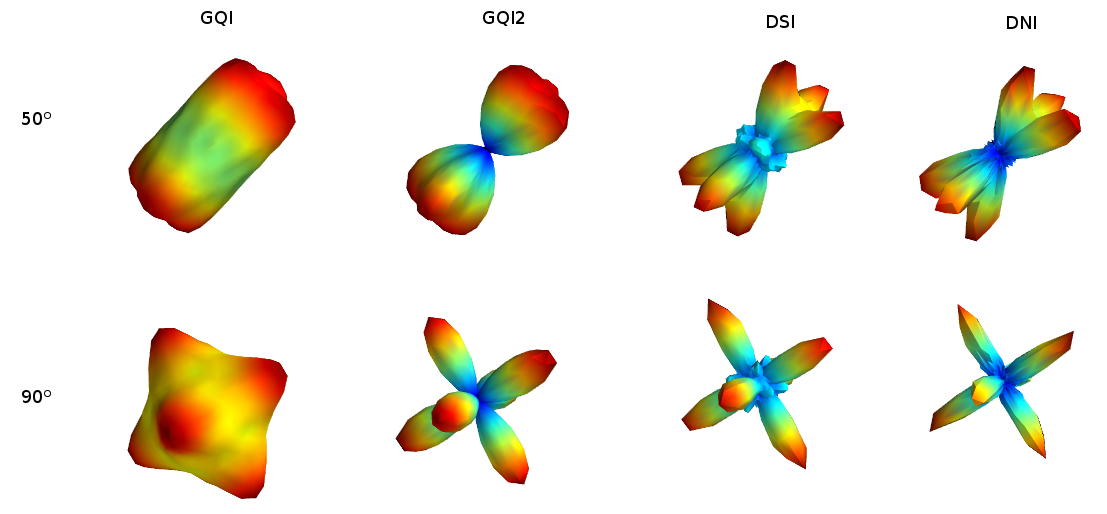
\includegraphics[scale=0.3]{last_figures/triple_crossing_gqi_gqi2_dsi_dni}
\par\end{centering}

\caption{Showing the ODFs from two randomly oriented simulated $3$-fibre crossings
at $50^{\circ}$(top) and $90^{\circ}$ angles between each pair of
fibres using different Cartesian lattice q-space reconstruction methods. }


\label{Flo:beautiful-triple-crossing}
\end{figure}


A new method for the calculation of the real ODF is proposed here.
This is based on the theoretical work done by Aganj et al.~\cite{aganj2010reconstruction}
and Canales-Rodriguez et al.~\cite{Canales-Rodriguez2009} using
two important theorems from Fourier Analysis
\begin{enumerate}
\item The Fourier transform of $P(\mathbf{r})r^{2}=-\nabla^{2}E(\mathbf{q})$
where $\nabla^{2}$ is the Laplacian operator (for proof see section
\ref{sub:Fourier-transform-ofPr2}).
\item For a symmetric function $E:\mathbb{R}^{3}\rightarrow\mathbb{R}$
and for the arbitrary unit vector $\hat{\mathbf{u}}$ we have $\intop_{0}^{\infty}E(r\hat{u})dr=\frac{1}{8\pi^{2}}\int\int_{\hat{\mathbf{u}}^{\perp}}E(q)\, q\, dq\, d\phi$
where $\hat{\mathbf{u}}^{\perp}$ is the plane perpendicular to $\hat{\mathbf{u}}$
(for proof see section \ref{sub:Radial-projection-of-symmetric}).
\end{enumerate}
From Eq.~\ref{eq:ODF_DSI} we see that the integration is over $P(r\hat{\mathbf{u}})r^{2}$
, therefore we can write

\selectlanguage{british}%
\begin{equation}
\psi_{DNI}(\hat{\mathbf{u}})=-\frac{1}{8\pi^{2}}\int_{\hat{\mathbf{u}}^{\perp}}\int_{0}^{\infty}\nabla^{2}E(q)\, q\, dq\, d\phi\label{eq:ODF_DNI}\end{equation}


\noindent where $\phi$ is the angular rotation component operating
on the plane perpendicular to $\hat{\mathbf{u}}$, \foreignlanguage{english}{$\nabla^{2}$
is the Laplacian operator and $E(q)=S(q)/S_{0}$ is the normalized
diffusion signal. Eq. \ref{eq:ODF_DNI} has the advantage that no
Fourier transform is necessary. We need however, a way to calculate
the Laplacian of the signal. This can be analytically derived for
a spherical grid \cite{aganj2010reconstruction} and we propose here
that it can be directly calculated in a cubic grid using the standard
3D discrete Laplacian filter which is given by the 3D kernel defined
by the following $3\times3\times3$ array: }

\selectlanguage{english}%
\[
\left[\left(\begin{array}{ccc}
0 & 0 & 0\\
0 & 1 & 0\\
0 & 0 & 0\end{array}\right),\left(\begin{array}{ccc}
0 & \:\,1 & \:\,0\\
1 & -6 & \:\,1\\
0 & \:\,1 & \:\,0\end{array}\right),\left(\begin{array}{ccc}
0 & 0 & 0\\
0 & 1 & 0\\
0 & 0 & 0\end{array}\right)\right].\]


\noindent This is a filter commonly used for image processing. From
now on when we use the Laplacian operator in order to measure the
directionality of the diffusion signal we will call this reconstruction
method Diffusion Nabla Imaging as nabla-squared ($\nabla^{2}$) is
the symbol for the Laplacian operator. In Fig.~\ref{Flo:beautiful-triple-crossing}
we present the ODFs from two randomly oriented simulated $3$-fibre
crossings at $50^{\circ}$ and $90^{\circ}$ angles between each other
using different grid based reconstruction methods. The parameters
used here are for DSI: radial sampling range $2.1-6$ with $0.2$
and Hanning filter width $36$, GQI: $\text{\ensuremath{\lambda}=1.2}$,
GQI2: $\lambda=3$ and DNI: radial sampling $0-5$ with $0.2$ steps.
All methods used the same reconstruction sphere with $642$ vertices
and $1,280$ faces. 


\subsection{Equatorial Inversion Transform}

We propose an important theoretical construction called the Equatorial
Inversion Transform (EIT) which creates a general formulation for
the interpretation of the directionality of the diffusion signal.
This idea is founded on two general properties of the diffusion signal:
(a) If we visualize the diffusion signal for a single fibre for all
gradient directions we see the generated shape to be lowest towards
the direction of the fibre and highest on the plane perpendicular
to that direction (see Fig.~\ref{Flo:single_fibre_spherical_grid}).
(b) The diffusion signal is additive i.e. $S(\hat{\mathbf{f}}_{1})+S(\hat{\mathbf{f}}_{2})=S(\hat{\mathbf{f}}_{1}+\hat{\mathbf{f}}_{2})$,
where $\hat{\mathbf{f}}_{1}$, $\hat{\mathbf{f}}_{2}$ are the unit
directions of the fibres. In simple terms the signal of 2-fibre crossing
can be decomposed linearly to the signals of the two fibres that create
the crossing. The same holds for any number of fibres in a crossing.

%
\begin{figure}
\begin{centering}
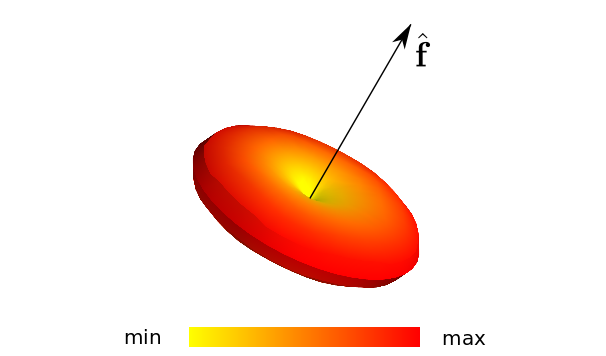
\includegraphics[scale=0.5]{last_figures/single_fiber_signal_sphere_grid2}
\par\end{centering}

\caption{The diffusion signal has the beautiful property that it is minimum
along the direction of a fibre with unit direction $\mathbf{\hat{\bm{f}}}$
and maximum along the equator defined by the plane perpendicular to
that fibre direction. This property is the basic inspiration behind
the EIT. In this picture the 3D surface plot of a simulated signal
for a spherical grid acquisition with b-value 2,000 is shown using
a yellow-red colourmap.}


\label{Flo:single_fibre_spherical_grid}
\end{figure}


These are two very important geometric properties of the signal that
we can try to exploit to its limit by calculating equatorial integrals
in order to identify the directionality of the signal. 

Apart from the visual confirmation, further supporting evidence that
equatorial integration is crucial for derivation of directionality
can be seen in Eq.~\ref{eq:ODF_DNI} where an equatorial integral
creates a connection between the real ODF and the signal. The Funk-Radon
Transform (FRT) used by \cite{Tuch2004} is another example where
equatorial integration is employed using the reconstruction sphere.
We will see next that DNI and FRT are just a subset of the EIT.

With EIT the most important goal is to try to identify the orientational
variation in the signal in the most accurate way by generating a spherical
density. However, it is possible to calculate additionally the classical
ODF as defined by Wedeen et al.~\cite{Wedeen}.

The EIT shown in Eq.~\ref{eq:ODF_EIT} consists of an integration
along the equator and along radial lines. A function $F$ of the signal
is multiplied by a radial weighting function $O$. This construction
is a generalization of the previous ODFs and it can support successfully
many different function families for $F$ and $O$ which can all more
or less accurately identify the directional distribution of the signal.
More precisely the EIT is defined as

\selectlanguage{british}%
\begin{equation}
\psi_{EIT}(\hat{\mathbf{u}})=\int_{\hat{\mathbf{u}}^{\perp}}\int_{0}^{\infty}F(E(q))O(q)dqd\phi\label{eq:ODF_EIT}\end{equation}


\begin{flushleft}
where $F$ could be for example any of the following functions\foreignlanguage{english}{\begin{equation}
F(E(q))=\begin{cases}
\,\,\,\,\,\,\,\,\, E(q) & (I)\\
-\nabla^{2}(E(q)) & (II)\\
\,\,\,\,\,\nabla^{4}(E(q)) & (III)\\
\,\,\,\,\,\ldots\end{cases}\label{eq:eit_operator}\end{equation}
and $O$ could be for example any of the following functions\begin{equation}
O(q)=\begin{cases}
1 & (0)\\
q & (1)\\
q^{2} & (2)\\
\ldots\end{cases}\label{eq:eit_radial_weighting}\end{equation}
}%
\begin{table}
\selectlanguage{english}%
\begin{centering}
\begin{tabular}{|c|c|c|c|}
\hline 
$F$ & $O$ & Name & Comment\tabularnewline
\hline
\hline 
$-\nabla^{2}(E(q))$ & $q$ & DNI$\equiv$EITL & \begin{tabular}{c}
calculates the real ODF without\tabularnewline
 the complications of the FFT\tabularnewline
\end{tabular}\tabularnewline
\hline 
$\nabla^{4}(E(q))$ & $q$ & EITL2 & high resolution at low angles\tabularnewline
\hline 
$E(q)$ & $q$ & EITS & \begin{tabular}{c}
impressive resolution without\tabularnewline
any preprocessing of the signal\tabularnewline
\end{tabular} \tabularnewline
\hline 
$E(q)$ & $1$ & 'QBI'-like & similar to the Funk Radon Transform\tabularnewline
\hline
\end{tabular}
\par\end{centering}

\caption{The Equatorial inversion transform (EIT) can be used to explain many
other reconstructions algorithms. }


\label{Tab:EIT_table}\selectlanguage{english}

\end{table}

\par\end{flushleft}

\selectlanguage{english}%
In Tab.~\ref{Tab:EIT_table} we see that by choosing different functions
for $F$ or $O$ we can generate both old and new distribution functions
on the sphere. With $F(E(q))=-\nabla^{2}(E(q))$ and $O(q)=q$ we
can generate $\psi_{DNI}$ which is theoretically identical to the
DSI real ODF($\psi_{DSI}$). If $F(E(q))=E(q)$ and $O(q)=1$ then
this is similar to the Funk Radon Transform (used in Q-ball imaging)
but applied to multiple spherical shells. However, we can also try
to use different functions like $F(E(q))=-\nabla^{4}(E(q))$ and $O(q)=q$
which can potentially increase the amount of directional information
beyond that of the standard ODFs. Before starting investigating the
realms of EIT we will first give a short overview of other methods
commonly found in the literature.


\subsection{Other methods}

Pickalov et al.~\cite{pickalov2006tra} proposed a new method for
reconstructing the diffusion propagator by applying an iterative inverse
Radon transform on measurements along many radial lines; computing
1D tomographic projections to reconstruct the 3D EAP. This technique
measures DW images along a few radial lines of q-space but still requires
hundreds of samples to reliably recover the EAP. Currently, to reconstruct
the EAP, the state-of-the-art model-free techniques apart from diffusion
spectrum imaging are hybrid diffusion imaging (HYDI)~\cite{wu2007hybrid}
and multiple q-shell diffusion propagator imaging (mq-DPI)~\cite{descoteaux2010multiple}.
HYDI acquires the signal values on five concentric spherical q-space
shells, then interpolates onto a cubic grid and applies the standard
Fourier transform in the same way as DSI. In mq-DPI the EAP is calculated
by solving Laplace's equation for the diffusion signal using a real
and symmetric modifi{}ed spherical harmonic basis. The EAP can be
found analytically by the inversion of a linear system using Laplace-Beltrami
regularization. In addition, Exact Q-ball imaging (EQBI)~\cite{canalesrodriguez2009mdq}
provides a different method to calculate the ODF analytically using
multiple spherical q-space shells. Similarly, Aganj et al.~\cite{Aganj2010},
proposed an analytical solution for the multi-shell case by incorporating
a mono-exponential or bi-exponential model (CSA-ODF). Another method
for finding a directional distribution on the sphere was proposed
by �zarslan et al.~\cite{ozarslan2006resolution} called the diffusion
orientation transform (DOT). This method calculates a different statistic
$P(r_{0}\mathbf{\hat{u}})$, the probability of finding a particle
initially at the origin at the point $r_{0}\mathbf{\hat{u}}$, using
spherical harmonics. Not surprisingly there is a relationship connecting
CSA with DOT which is \foreignlanguage{british}{\begin{equation}
\psi_{CSA}(\hat{\mathbf{u}})=\int_{0}^{\infty}DOT(r\hat{\mathbf{u}})r^{2}dr\label{eq:CSAandDOT}\end{equation}
}

\selectlanguage{british}%
J\foreignlanguage{english}{ansons et al.~\cite{JansonsPAS2003} proposed
a different function on the sphere than the ODFs described above,
to be used on data sets acquired on a single spherical q-space shell.
They called this spherical function persistent angular structure (PAS).
This method has very good angular resolution. It uses the principle
of maximum entropy however, it is rather slow as it nonlinear fitting
is used in order to identify many parameters. PAS is a statistic on
the sphere defined as $PAS(\hat{\mathbf{u}})=\exp(\lambda_{0}+\sum_{j=1}^{N}\lambda_{j}\cos(\mathbf{q}_{j}\cdot k\hat{\mathbf{u}}))$
where $\lambda$ are the unknown parameters, $k$ is constant and
$N$ is the number of DWIs. The relationship $\int PAS(\hat{\mathbf{u}})\exp(i\mathbf{q}_{j}\cdot k\hat{\mathbf{u}})d\hat{\mathbf{u}}=E(\mathbf{q}_{j})$
provides the bridge between PAS and the diffusion signal ($E(\mathbf{q})$).}

\selectlanguage{english}%
The first publication of using spherical harmonic expansions with
diffusivity profiles, which are now quite common in the literature,
was by Alexander et al.~\cite{alexander2002detection}. Q-ball imaging
was introduced by Tuch~\cite{Tuch2004} and a new ODF defined as
$\psi(\mathbf{\hat{u}})=\frac{1}{Z}\int_{0}^{\infty}P(r\mathbf{\hat{u}})dr$
where $Z$ is a normalization constant. It was later provided for
Q-Ball imaging a fast and analytical solution using spherical harmonics
(SH) and Laplace-Beltrami regularization \cite{Descoteaux2007}. Tournier
et al. \cite{tournier2004direct}, \cite{Tournier2007} introduced
a spherical deconvolution method where first the SH coefficients were
estimated, then single fiber ODFs were used as a deconvolution kernel
estimated from the real data. Then, the sharper fODF (fiber orientation
distribution function) was obtained by a simple linear transformation
\cite{descoteaux2007deterministic}. Other deconvolution approaches
were proposed in \cite{sakaie2007objective} and \cite{yeh2011estimation}.

On Tensor related methods we have the classical Single Tensor \cite{Basser1994},
Sticks and Ball\cite{Behrens2007NeuroImage}, Multi-Tensor \cite{pasternak2008variational},
\cite{liu2004characterizing} and Higher Rank Tensors \cite{ozarslan2003generalized},
\cite{barmpoutis2009regularized}. In addition there are also model
based methods which try to calculate non-Gaussian properties, for
example the Kurtosis Tensor~\cite{jensen2005diffusional},~\cite{lu2006three}
which is used in Diffusion Kurtosis Imaging (DKI).

Finally, new model-based methods are emerging which are trying to
calculate statistics like the axonal thickness distribution from dMRI
data sets. These are usually based on model free and restricted components;
CHARMED~\cite{assaf2005composite}, \cite{assaf2004new}, AxCaliber~\cite{assaf2008axcaliber}
and the orientation invariant ActiveAx \cite{alexander2010orientationally}
are some well known methods of this type. Q-space Imaging (QSI) can
be used to identify distributions of axon-diameter too \cite{ong2010quantifying}.


\subsection{Implementation }

%
\begin{figure}
\begin{centering}
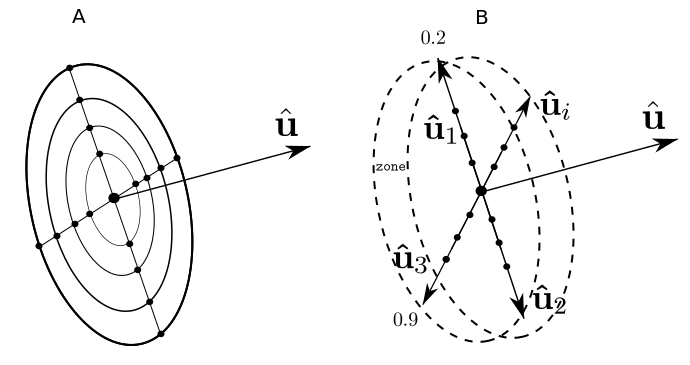
\includegraphics[scale=0.5]{last_figures/fast_DNI}
\par\end{centering}

\caption{A: Standard EIT. B: Fast EIT. Fast EIT is an order of magnitude faster
than standard EIT. The key idea here is that we can reduce computations
by storing the sum of the radial integrals for every vertex in the
reconstruction sphere and then we can also precompute the indices
of the vertices that are near the equator of every vertex (inside
an equatorial zone).}


\label{Flo:sEITvsEIT}
\end{figure}



\subsubsection{Standard EIT\label{sub:Standard-EIT}}

Eq.~\ref{eq:ODF_DNI} and \ref{eq:ODF_EIT} can be implemented in
a standard way by evaluating the 3D signal on the grid multiple times
for every direction $\hat{\bm{u}}$ as shown in Fig.~\ref{Flo:sEITvsEIT}A.
This suggests that if for example we use a reconstruction sphere of
$642$ vertices and the signal is centered inside a cubic grid of
size $17\times17\times17$ where the radial integration ($q$) takes
place in $30$ steps and the equatorial ($\phi$) in $63$ steps,
then we need to interpolate $642\times30\times30\simeq1.2$ million
times on the cubic grid. For this reason we invented Fast EIT, a new
method that needs an order of magnitude less evaluations.

In this document whenever we use the prefix 's' in front of a method
it means it was calculated with the standard EIT algorithm. For example
if standard EIT is used for DNI we will write sDNI or sEITL. ('L'
stands for 'Laplacian' or 'Nabla'). Of course, sDNI and sEITL are
equivalent.


\subsubsection{Fast EIT}

A much faster algorithm than the standard EIT is described here. The
main idea is that we can store the sum of the radial integrals for
every vertex in the reconstruction sphere so we can then precompute
the indices of the vertices that are near the equator of every vertex
(inside an equatorial zone). This becomes clear in see Fig.~\ref{Flo:sEITvsEIT}B.
Following these calculations, the spherical distribution function
can be approximated with much less operations. The full algorithm
is given in Alg.~\ref{Alg:Fast_EIT}. The input is the vertices $\hat{\bm{u}}_{i}$
of the reconstruction sphere and the normalized signal $E.$ Then,
for every point of the reconstruction sphere $\hat{\bm{u}}_{i}$,
we save the indices of the vertices $j$ of $\hat{\bm{u}}_{j}$, which
are inside an equatorial zone, in list $J_{i}$. The width of the
equatorial zone $z$ is a constant set empirically to $5^{\circ}$
. If a very highly dense reconstruction sphere is used with more than
$642$ vertices, which is the one we used, then the zone can be smaller.
That can potentially increase the angular resolution of the method.

%
\begin{algorithm}
\textbf{Input} $U=\{\hat{\bm{u}}_{1}\ldots\hat{\bm{u}}_{m}\}$, E\\
\textbf{Output} $\bm{\psi}_{EIT}$\\
\\
\textbf{For} $\hat{\bm{u}}_{i}$ in $U$ \textbf{Do}\\
\hspace*{2em} $J_{i}=\{j : |\arccos(\hat{\bm{u}}_{i}\cdot\hat{\bm{u}}_{j})|\leq z \}$\\
\textbf{EndFor} \\
\textbf{For} $\hat{\bm{u}}_{i}$ in $U$ \textbf{Do}\\
\hspace*{2em} $\mathbb{B}(\hat{\bm{u}}_{i})=\sum_{k=0}^{n}F(E(q_{k}\hat{\bm{u}}_{i}))O(q_{k}\hat{\bm{u}}_{i})$\\
\hspace*{4em} where $F(E(q_{k}\hat{\bm{u}}_{i}))$ is interpolated on the lattice.\\
\hspace*{2em} $\psi_{EIT}(\hat{\bm{u}}_{i})=\frac{1}{N_i}\sum_{j\in J_i}\mathbb{B}(\hat{\bm{u}}_{j})$\\ 
\hspace*{4em} where $N_i$ is the number of indices in $J_i$.\\
\textbf{EndFor}

\caption{Fast Equatorial Inversion Transform}


\label{Alg:Fast_EIT}
\end{algorithm}


At the next stage we calculate sums along every radius on the direction
of $\hat{\bm{u}}_{i}$ in the following way: $\mathbb{B}(\hat{\bm{u}}_{i})=\sum_{k=0}^{n}F(E(q_{k}\hat{\bm{u}}_{i}))O(q_{k}\hat{\bm{u}}_{i})$
and obtain the final EIT ODF as the average of the sums in the equator
$\psi_{EIT}(\hat{\bm{u}}_{i})=\frac{1}{N_i}\sum_{j\in J_i}\mathbb{B}(\hat{\bm{u}}_{j})$
where $F$ is evaluated with trilinear for example interpolation on
the lattice and $N_{i}$ is the number of indices in $J_{i}.$

In section \ref{sub:Multi-fiber-Simulations} the standard EITL (sEITL)
is compared with fast EITL. In Fig.~\ref{Flo:FastvsStandardEITL}
it is shown that the fast EIT has very similar results with the standard
EIT. From now on whenever we write EIT we refer to the fast version. 


\subsection{Peak Finding\label{sub:Peak-Finding}}

After we have generated the ODFs we need to find the peaks (local
maxima) from which we can easily approximate the direction of the
fibres. Peak finding is not trivial if there are many local maxima
in the ODFs or the ODFs are noisy. Here we present an algorithm (see
Alg.~\ref{Alg:PeakFinding}) which reduces the amount of small local
variations and returns a number of sorted peaks and their indices
in the reconstruction sphere. The input of this algorithm is $\bm{\psi}$
(ODF) and the faces of a symmetric on the z-axis evenly distributed
sphere (see Fig.~\ref{Flo:sphere_642}C).

%
\begin{algorithm}
\textbf{Input} ODF $\bm\psi$, faces $\Phi$ \\
\textbf{Output} peaks $P$ and indices $I$ \\
\\
\textbf{For} face $\Phi_i$ in $\Phi$ \textbf{Do}\\
\hspace*{2em} $f_0,f_1,f_2 = \Phi_i$ \\	
\hspace*{2em} $d_0,d_1,d_2 =\bm{\psi}[f_0],\bm{\psi}[f_1],\bm{\psi}[f_2]$ \\	
\hspace*{2em} \textbf{If} $d_0 \geq d_1$ \textbf{and} $d_2$ \textbf{Do}\\
\hspace*{4em} $P[f_1]=P[f_2]=0$ \\
\hspace*{4em} \textbf{continue} \\
\hspace*{2em} \textbf{EndIf} \\
\textbf{EndFor}

\caption{Peak Finding with a Symmetric Ordered Sphere}

\label{Alg:PeakFinding}
\end{algorithm}


We have used a triangulation of the unit sphere (which we refer to
simply as 'sphere') obtained by triangular subdivision of a regular
icosahedron. It is symmetric over the z-axis, i.e.~for each vertex
$(x,\, y,\, z)$ there is a corresponding vertex $(x,\, y,\,-z)$
in the opposite hemisphere. The same sphere was used in \cite{Yeh2010}
for GQI reconstructions. Every face (triangle) corresponds to a list
of the $3$ indices of the $3$ vertices on the sphere. The idea here
is that we can travel from face to face and nullify all points on
a face which are lower that the higher value of the face. At the end
only local maxima will survive the procedure. The algorithm is presented
in detail in Alg.~\ref{Alg:PeakFinding}.

The sphere we use is of course discrete and therefore it adds some
constraints on the angular resolution (worst case$\pm4.96^{\circ}$)
of the peaks found from the ODF. In addition, the proposed Peak Finding
algorithm can reduce slightly more the angular resolution. For example,
in Fig.~\ref{Flo:sphere_642}A, B we show that if point \textbf{a}
was a local maxima then only points \textbf{b} could be alternative
local maxima for \textbf{a} but none of the unlabeled points could
be a second peak. Nevertheless, we found Alg.~\ref{Alg:PeakFinding}
to be extremely useful and fast. The same algorithm was used also
in \cite{Yeh2010} but it was not documented as such.

%
\begin{figure}
\begin{centering}
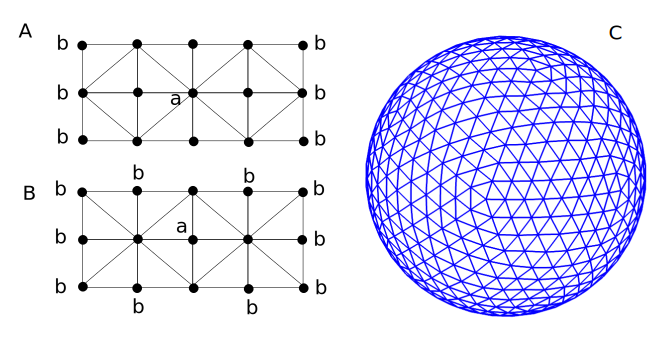
\includegraphics[scale=0.6]{last_figures/peak_finding_sphere}
\par\end{centering}

\centering{}\caption{A and B: Each point \textbf{a} is a local maximum for all its neighboring
faces, then only at \textbf{b} are other possible local maxima. This
simple illustration shows that the triangulation of the sphere is
important for the determination of closed peaks and that peaks which
belong to the same triangle cannot be determined. C: the sphere used
for ODF reconstructions consisting of $642$ vertices and $1,280$
faces produced by subdivisions of the icosahedron.}
\label{Flo:sphere_642}
\end{figure}



\subsection{Spherical Angular Smoothing\label{sub:Spherical-Angular-Smoothing}}

All current non-parametric dMRI reconstruction algorithms use some
type of {}``smoothing'' to reduce the effect of noise in the real
data sets. DSI uses a Hanning filter and then avoids sampling from
low values in \textbf{r}-space. In GQI, smoothing is controlled from
a scalar parameter; the diffusion sampling length and in spherical
harmonic inversion methods \cite{Descoteaux2007MagResMed}, \cite{aganj2010reconstruction}
the amount of smoothing is controlled by using only a number of the
first components of the SH series. 

All these approaches smooth and calculate the ODFs simultaneously.
Our appoach differs in that we propose that the ODF is first calculated
and then smoothed. For example, using the operator shown below in
matrix form\[
W=\exp(\frac{U\cdot U^{T}}{\sigma})\]


\noindent where $U$ is the an $N\times3$ matrix holding the $N$
points of the ODF reconstruction sphere and $\sigma$ is a smoothing
parameter acting like the variance. At the next step we can smooth
any ODF($\bm{\psi}$) creating a new ODF($\bm{\psi}'$) in the following
way\begin{equation}
\bm{\psi}'=\bm{\psi}\cdot\frac{W}{\sum_{j}W_{j}}\label{eq:spherical_gaussian_angular_smoothing}\end{equation}


\noindent where $j$ denotes row indexing, $\sum_{j}W_{j}$ acts as
a normalization for the angular weighting $W$, $\bm{\psi}$ is the
initial ODF and $\bm{\psi}'$ is the smoothed ODF . The advantage
of this method is that it is more comprehensive and direct. It also
uses information from all directions simultaneously. Similar operators
can be constructed that weight more lower or higher peaks. The operator
shown here weighs more peaks that are closer in angular distance.
In Fig.~\ref{Flo:Smoothing_Example} we see the effect of this equation
on a simulated triple-fibre crossing; distorted with Gaussian noise
with SNR $20$ and reconstructed as an EITL density function. The
simulation was used using a Sticks and Ball model with diffusivity
value $0.0015$ and S0=$100$.

%
\begin{figure}
\begin{centering}
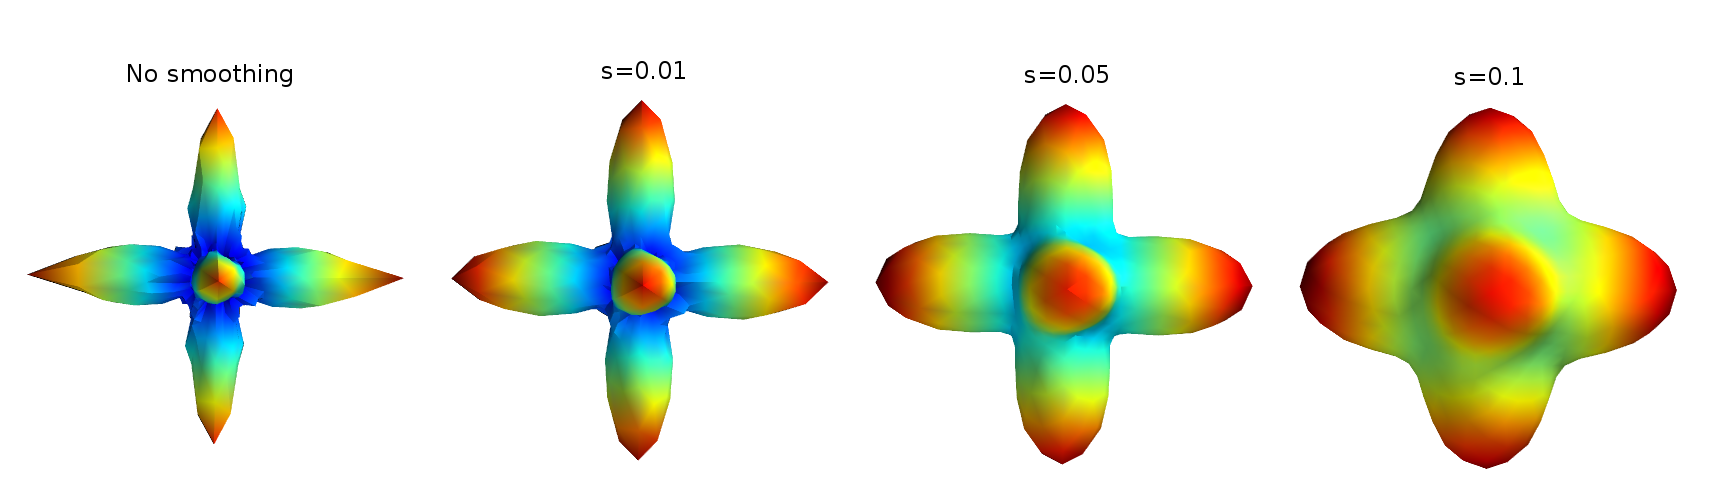
\includegraphics[scale=0.2]{last_figures/triple_crossing_laplacian_snr20}
\par\end{centering}

\caption{An example of spherical angular Gaussian smoothing applied with different
smoothing factors on the ODF of a triple-fibre crossing on the left. }


\centering{}\label{Flo:Smoothing_Example}
\end{figure}


We can easily observe that when we increase the smoothing factor $\sigma$,
small noisy peaks, as seen in the center of the unsmoothed spherical
function, can easily be removed. However, with too much smoothing
even the strongest peaks can lose their definition. This spherical
operator can help to set the trade-off between noise and signal and
it can also simplify the peak finding process, i.e.~finding the underlying
primary fibre directions as this problem is much easier on smooth
surfaces.

Finally, decoupling the smoothing from the reconstruction step gives
an important advantage: reducing the effect of the noise to our data
more strongly and independently. Many spherical operators can be added
as plugins independently of the reconstruction phase, and these can
work with any function on the sphere (see Eq.~\ref{eq:spherical_gaussian_angular_smoothing}).


\subsection{Comparisons and Results}

Validation of reconstruction and tractography algorithms is not straightforward
due to the lack of relevant gold standards. Simulated voxels and software
phantoms are a useful way to overcome this difficulty and test new
methods. Following the simulation results, we show results with real
human data sets.


\subsubsection{Multi-fibre Simulations\label{sub:Multi-fiber-Simulations}}

%
\begin{figure}
[th!]

\centering{}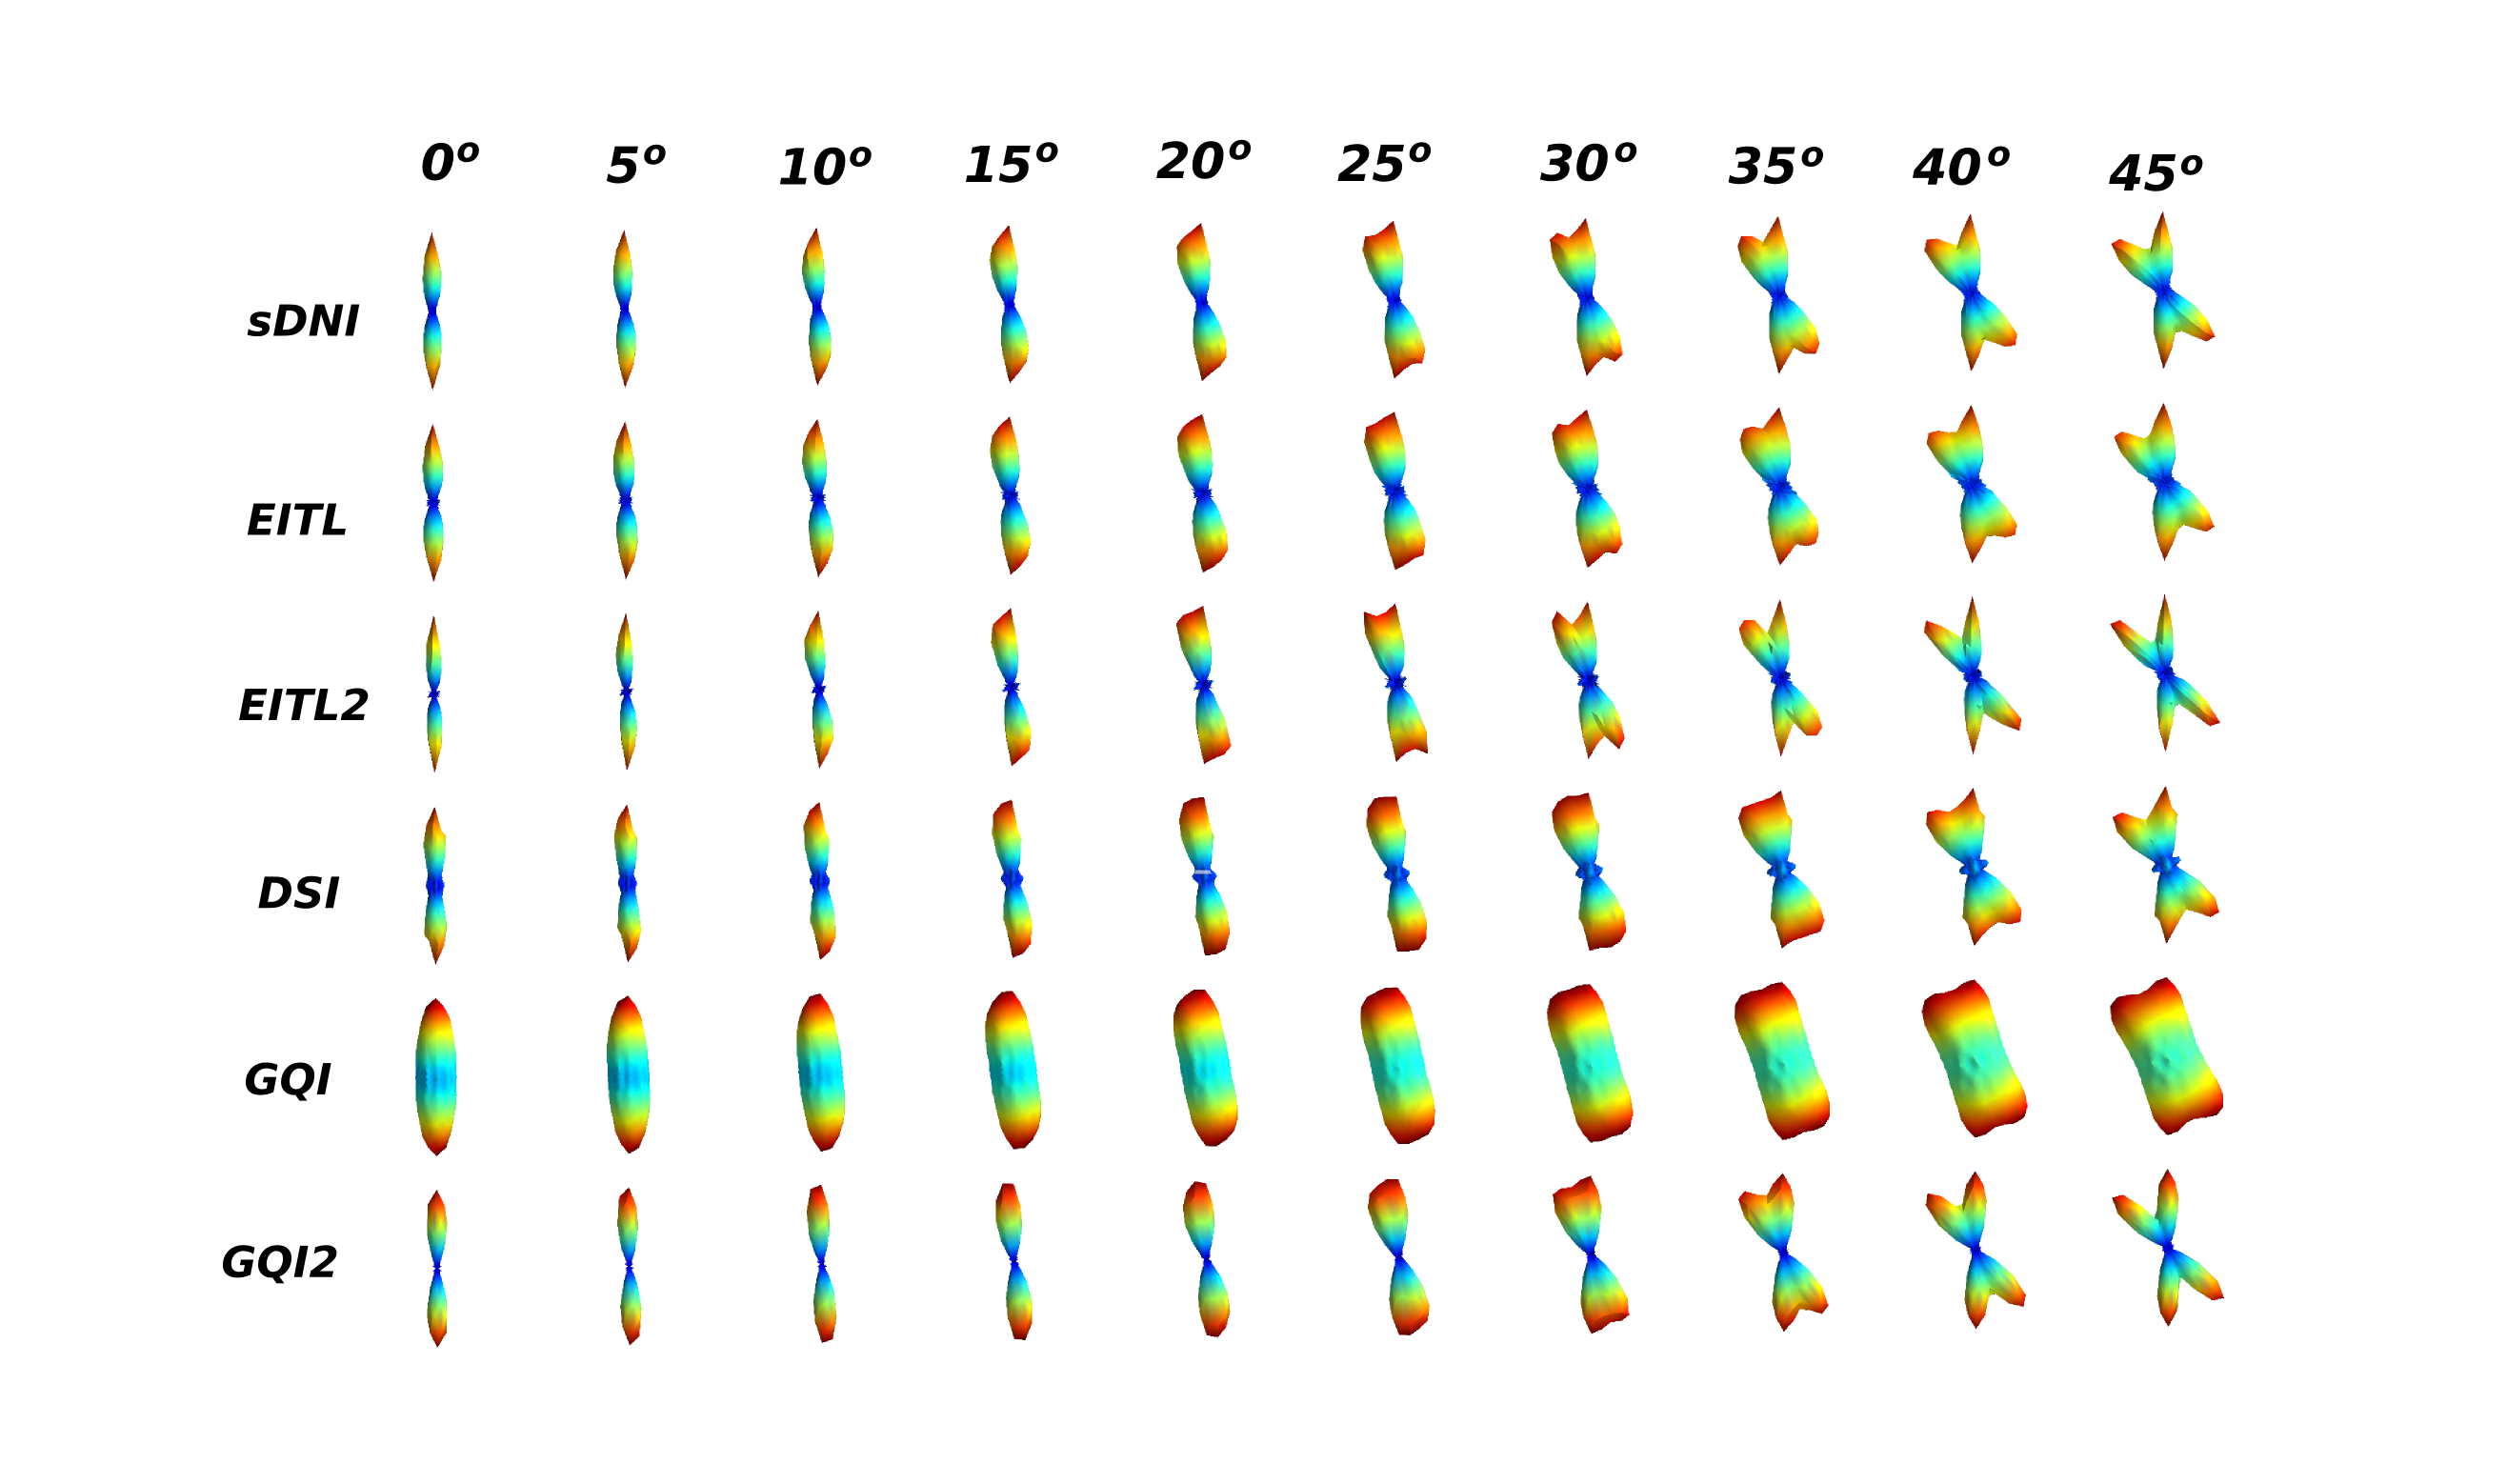
\includegraphics[scale=0.6]{last_figures/low_angles_with_labels}\caption{Visualizing ODFs created from different reconstruction methods sDNI
(sEITL), EITL, EITL2, DSI, GQI and GQI2. We can see that standard
DNI (sDNI), EITL and EITL2 can resolve the correct angular fibre directions
at lower angles than the other methods. For example see column at
angle of $25^{\circ}$. }
\label{Flo:multi-fibre-sims}
\end{figure}


For single voxel simulations we used the model proposed in Behrens
et al.~\cite{Behrens2007NeuroImage}; the multi-compartment model
also known as Sticks and Ball which simulates the diffusion signal
as\begin{equation}
S_{i}=S_{0}((1-\sum_{j=1}^{N}f_{j})\exp(-b_{i}d)+\sum_{j=1}^{N}f_{j}\exp(-b_{i}d\cos(\theta_{ij})^{2}))\label{eq:sticks_ball_eq}\end{equation}
\noindent where $\theta_{ij}$ is the angle between gradient direction
$\mathbf{\hat{g}}_{i}$ and fibre (stick) unit direction $\mathbf{\hat{u}}_{j}$.
The amount of representation for every fibre is given by $f$ and
$d$ is the diffusivity value for the entire model. A Multi Tensor
\cite{liu2004characterizing} approach was also created for software
phantoms using the formula\foreignlanguage{british}{\begin{equation}
S_{i}=S_{0}\sum_{j=1}^{N}\exp(-b\mathbf{\hat{g}}^{T}D_{j}\mathbf{\hat{g}})\label{eq:multitensor}\end{equation}
where $D_{j}$ is the diffusion tensor for every fibre $j$.}

In Fig.~\ref{Flo:multi-fibre-sims} we present the outcome of an
experiment of two crossing fibres using different reconstruction methods:
sDNI (sEITL), EITL, EITL2, DSI, GQI and GQI2. These are based on simulations
of 2-fibre crossings from $0^{\circ}$ to $90^{\circ}$ using Eq.~\ref{eq:sticks_ball_eq}
with diffusivity value of $1.5\times10^{-3}$ \foreignlanguage{british}{$\textrm{mm}^{2}/\textrm{sec}$}
and 257 b-values with maximum b-value $11,000$. However, all these
methods will perform accurately beyond $50^{\circ}$ therefore in
this figure we present only the lower angles. We can see that sDNI,
EITL and EITL2 performed better than the other methods. Especially
EITL2 was able to resolve crossing at $25^{\circ}$ which is lower
than the accuracy resolved in the current state of the art methods.
In order to confirm this fascinating result we created a more general
experiment with many iterations (of 2-fibre and 3-fibre crossings)
which is presented below.

A comparison metric is needed in order to evaluate the new and old
reconstruction methods discussed in this chapter. The standard procedure
is to calculate the similarity between the measured and simulated
ground truth data sets. We want to calculate the angular precision
of the ODFs from simulations derived from Eq.~\ref{eq:sticks_ball_eq}.
We define a new similarity metric called Angular Similarity (AS) which
computes the cosine distance of the best match between the set of
measured fibre orientations and the known set of simulated fibres.
This metric will be used to compare 2-fibre and 3-fibre crossings.
AS is $0$ when there is no match i.e. angular distance is $0$, $1$
when one fibre is matched ($0^{\circ}$), $2$ when two fibres are
matched and $3$ when three fibres are matched. In table \ref{Tab:AS_behaviour}
we show a few examples of AS behaviour with simple unit vector sets. 

%
\begin{table}
\begin{centering}
\begin{tabular}{|c|c|c|}
\hline 
Known & Measured & AS\tabularnewline
\hline
\hline 
$(1,0,0),(0,1,0)$ & $(0,0,1)$ & $0$\tabularnewline
\hline 
$(1,0,0),(0,1,0)$ & $(0,1,0)$ & $1$\tabularnewline
\hline 
$(1,0,0),(0,1,0)$ & \selectlanguage{british}%
$(0,\nicefrac{\sqrt{2}}{2},\nicefrac{\sqrt{2}}{2})$\selectlanguage{english}
 & \selectlanguage{british}%
$\nicefrac{\sqrt{2}}{2}$\selectlanguage{english}
\tabularnewline
\hline 
$(1,0,0),(0,1,0),(0,0,1)$ & $(1,0,0),(0,0,1)$ & $2$\tabularnewline
\hline
\end{tabular}
\par\end{centering}

\caption{Examples of angular similarity (AS) behaviour with simple unit vector
sets.}


\label{Tab:AS_behaviour}
\end{table}


If our ground truth set consists of $g=[(1,0,0),(0,1,0)]=[g_{0},g_{1}]$
and the measured set consists of $m=[(0,0,1)]$ then AS=$0$. If the
measured set was $m=[(0,\nicefrac{\sqrt{2}}{2},\nicefrac{\sqrt{2}}{2})]=[m_{0}]$
then AS\foreignlanguage{british}{ is$\nicefrac{\sqrt{2}}{2}$. This
is because according to the AS definition we have $AS(g,m)=\max(|g_{0}\cdot m_{0}|,|g_{1},m_{0}|)$.
Which is equal to $\nicefrac{\sqrt{2}}{2}$.}

\selectlanguage{british}%
\noindent~If $g=[(1,0,0),(0,1,0)]=[g_{0},g_{1}]$ and $m=g$ then
$AS(g,m)=\max(|g_{0}\cdot m_{0}|+|g_{1}\cdot m_{1}|,|g_{0}\cdot m_{1}|+|g_{1}\cdot m_{0})=2.$
We created an experiment where we set two fibres at an increasing
angle of \foreignlanguage{english}{$2.5^{\circ}$}from $0^{\circ}$
to $90^{\circ}$ and then rotate them uniformly around $200$ random
axes. This operation produces $7,400$ simulated ODFs and the results
are shown in Fig.~\ref{Flo:2_100} and Fig.~\ref{Flo:2_20} with
different signal to noise ratio. For these simulations noise was normally
distributed. What we see in the figures is the average angular similarity
where the average is calculated from the $200$ random orientations
for the same angle.

\selectlanguage{english}%
%
\begin{figure}
\begin{centering}
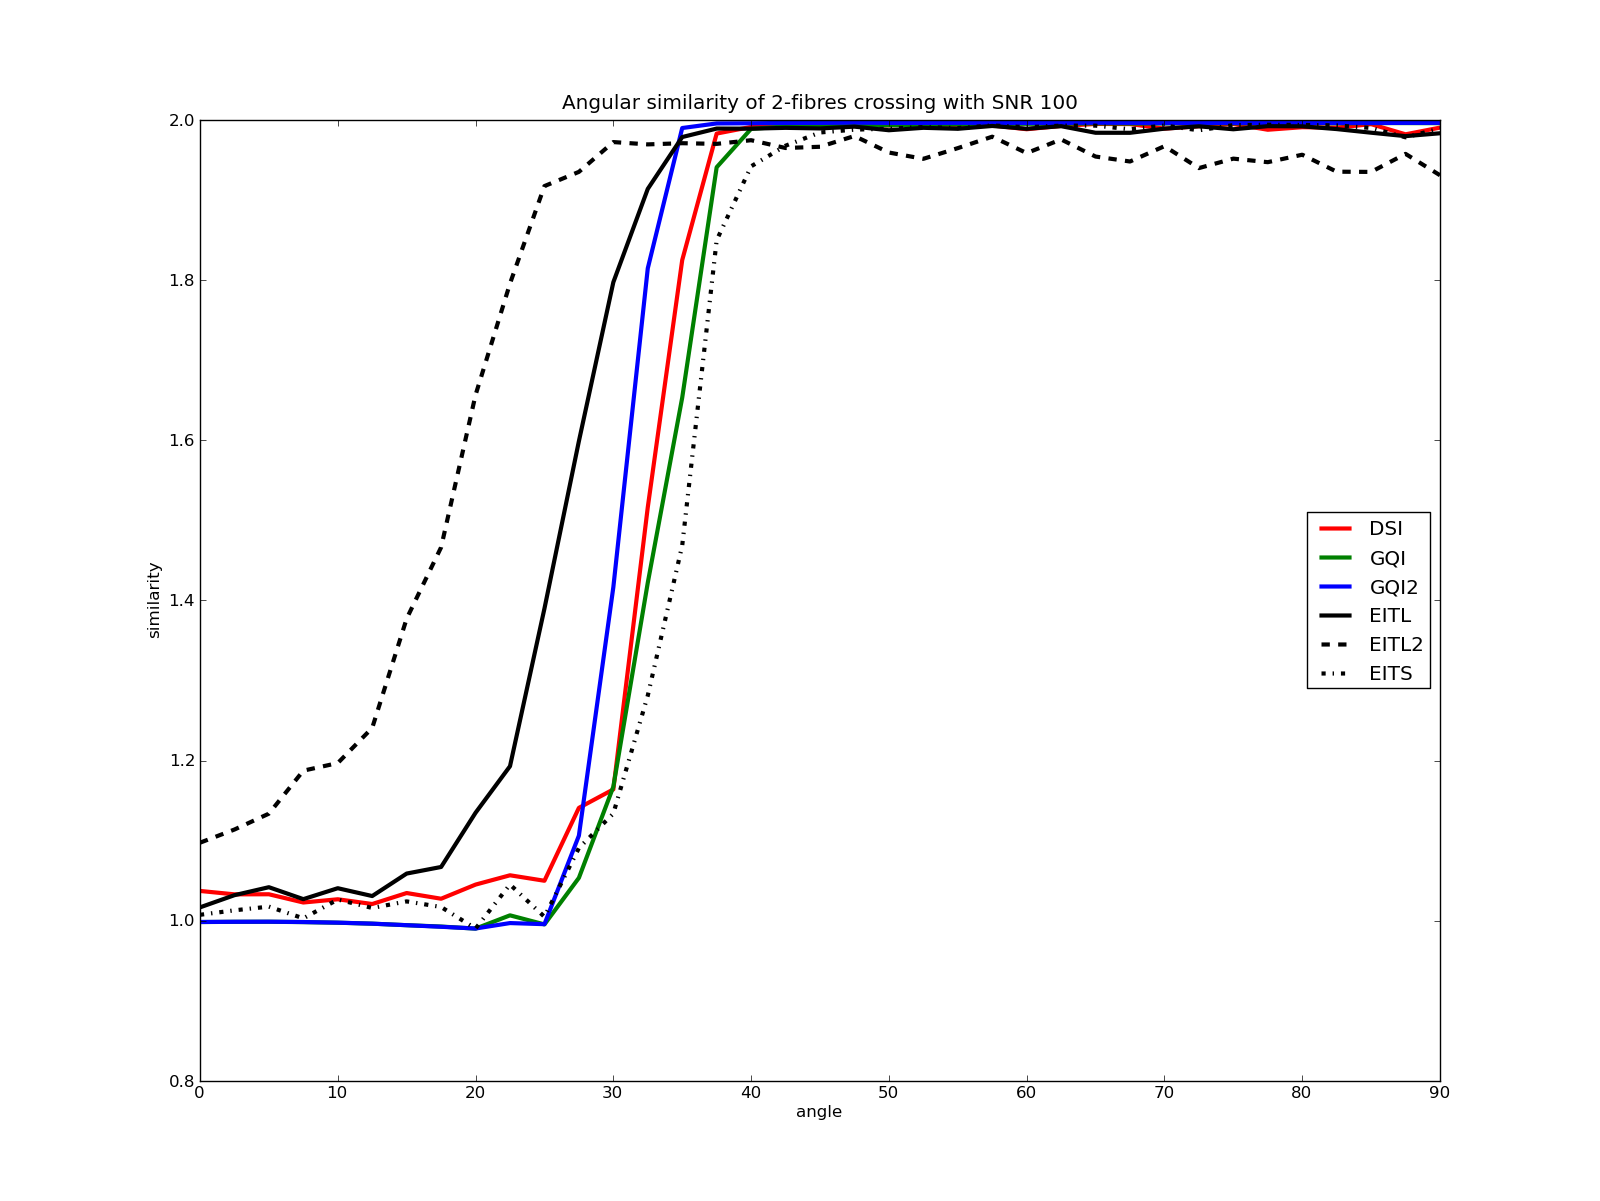
\includegraphics[scale=0.5]{last_figures/2_100}
\par\end{centering}

\caption{Average angular similarity of 2-fibre crossings with SNR 100}


\label{Flo:2_100}
\end{figure}


We can easily observe in Fig.~\ref{Flo:2_100} that EITL2 can resolve
more accurately fibre crossings at low angles and continues to perform
well even at higher angles $>50^{\circ}$ . EITL performs better than
DSI, GQI, GQI2 and EITS at low angles and very well at high angles
as well. GQI2 performs better than DSI, GQI, and ETS. It is also impressive
that EITS can have such a good performance although it is such a simple
operation. In summary we see from the graphs that EITL2$>$EITL$>$GQI2$>$DSI$>$GQI$>$EITS
where $>$ means higher average angular similarity. The same pattern
takes place even when we increase the noise level see for example
Fig.~\ref{Flo:2_20}. We will see next that the same pattern appears
even with 3-fibre crossings and high levels of noise.

%
\begin{figure}
\begin{centering}
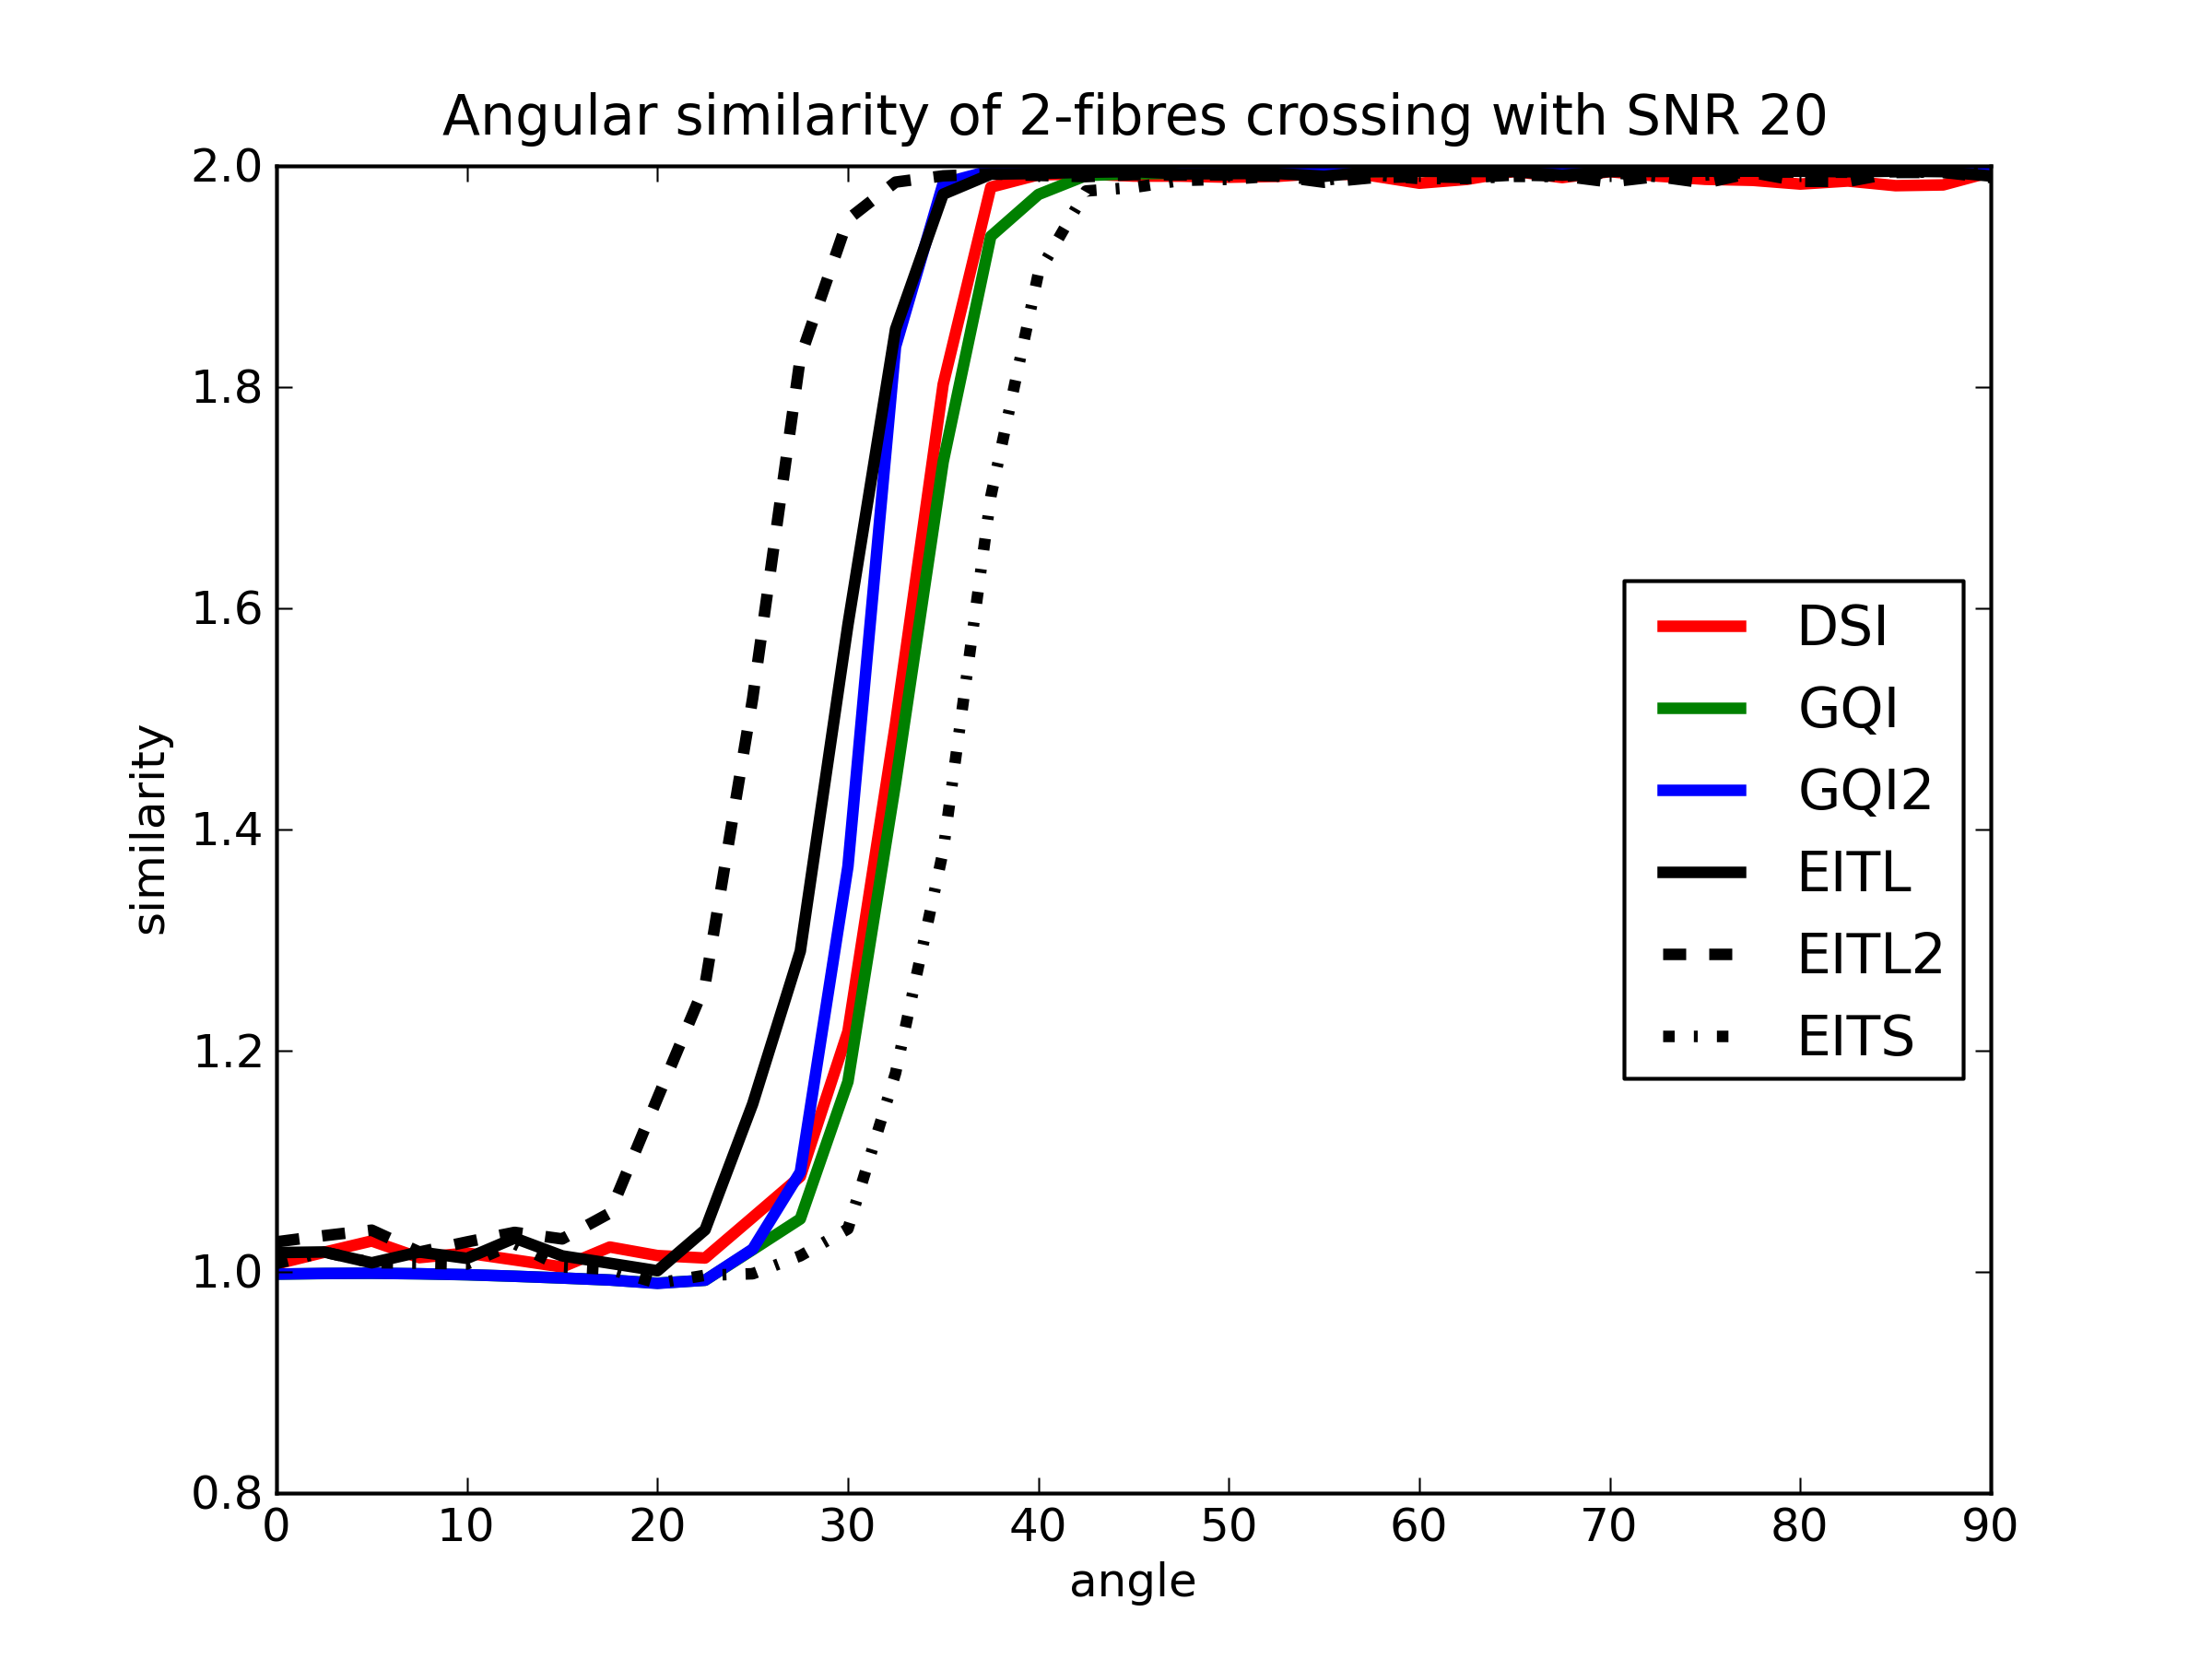
\includegraphics[scale=0.5]{last_figures/2_20}
\par\end{centering}

\caption{Average angular similarity of $2$-fibre crossings with SNR 20. }


\label{Flo:2_20}
\end{figure}


We also measured the accuracy in $3$-fibre crossings. In this experiment
the $3$-fibres will always have the same angular distance between
each other. That distance will increase from \foreignlanguage{british}{$0^{\circ}$
to $90^{\circ}$ }with steps of $2.3^{\circ}$ on average and all
$3$ fibres will be reoriented $200$ times. That gave $8,000$ simulated
crossings. 

%
\begin{figure}
\begin{centering}
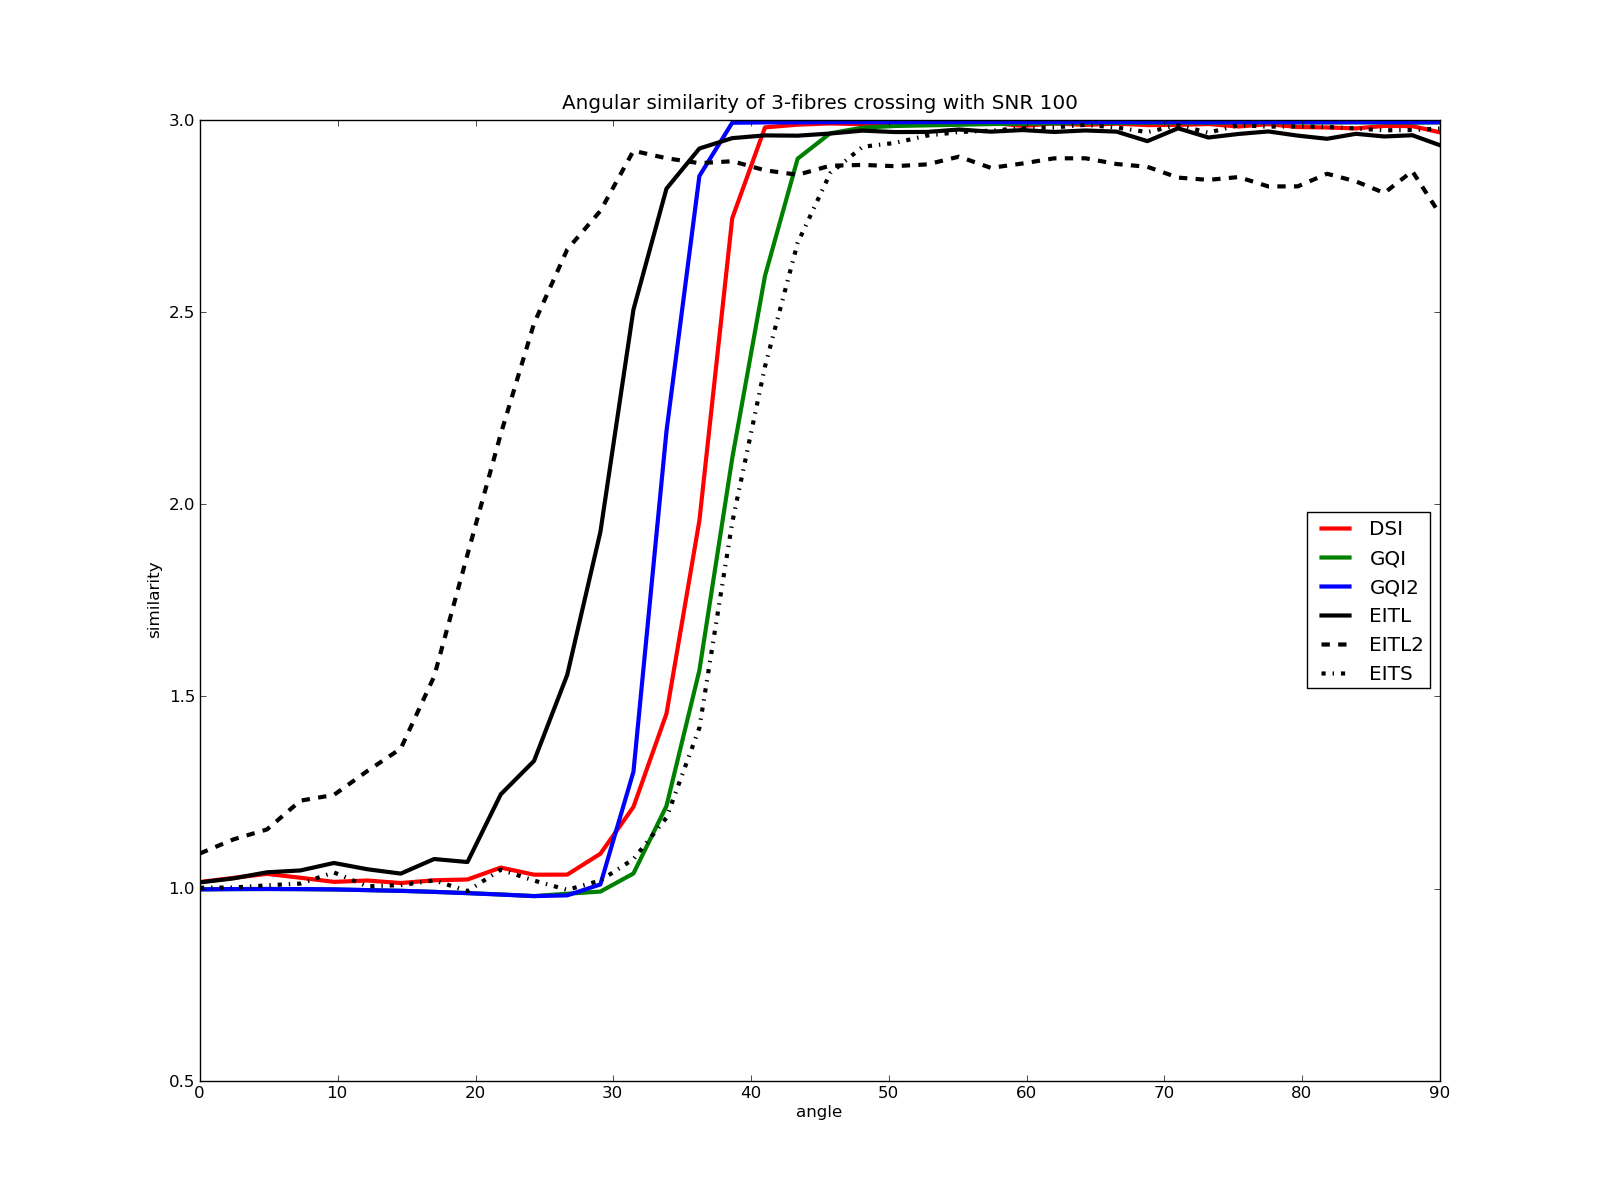
\includegraphics[scale=0.5]{last_figures/3_100}
\par\end{centering}

\caption{Average angular similarity of $3$-fibre crossings with SNR $100$.}


\label{Flo:3_100}
\end{figure}


The results of the 3-fibre crossings shown in Fig.~\ref{Flo:3_100}
and Fig.~\ref{Flo:3_20} were very similar to those of the 2-fibre
crossings; EITL2 performed better at low angles, showing slightly
reduced performance at high angles. EITL performed better with low
angles than the rest of the methods, having also high accuracy on
larger angles.

%
\begin{figure}
\begin{centering}
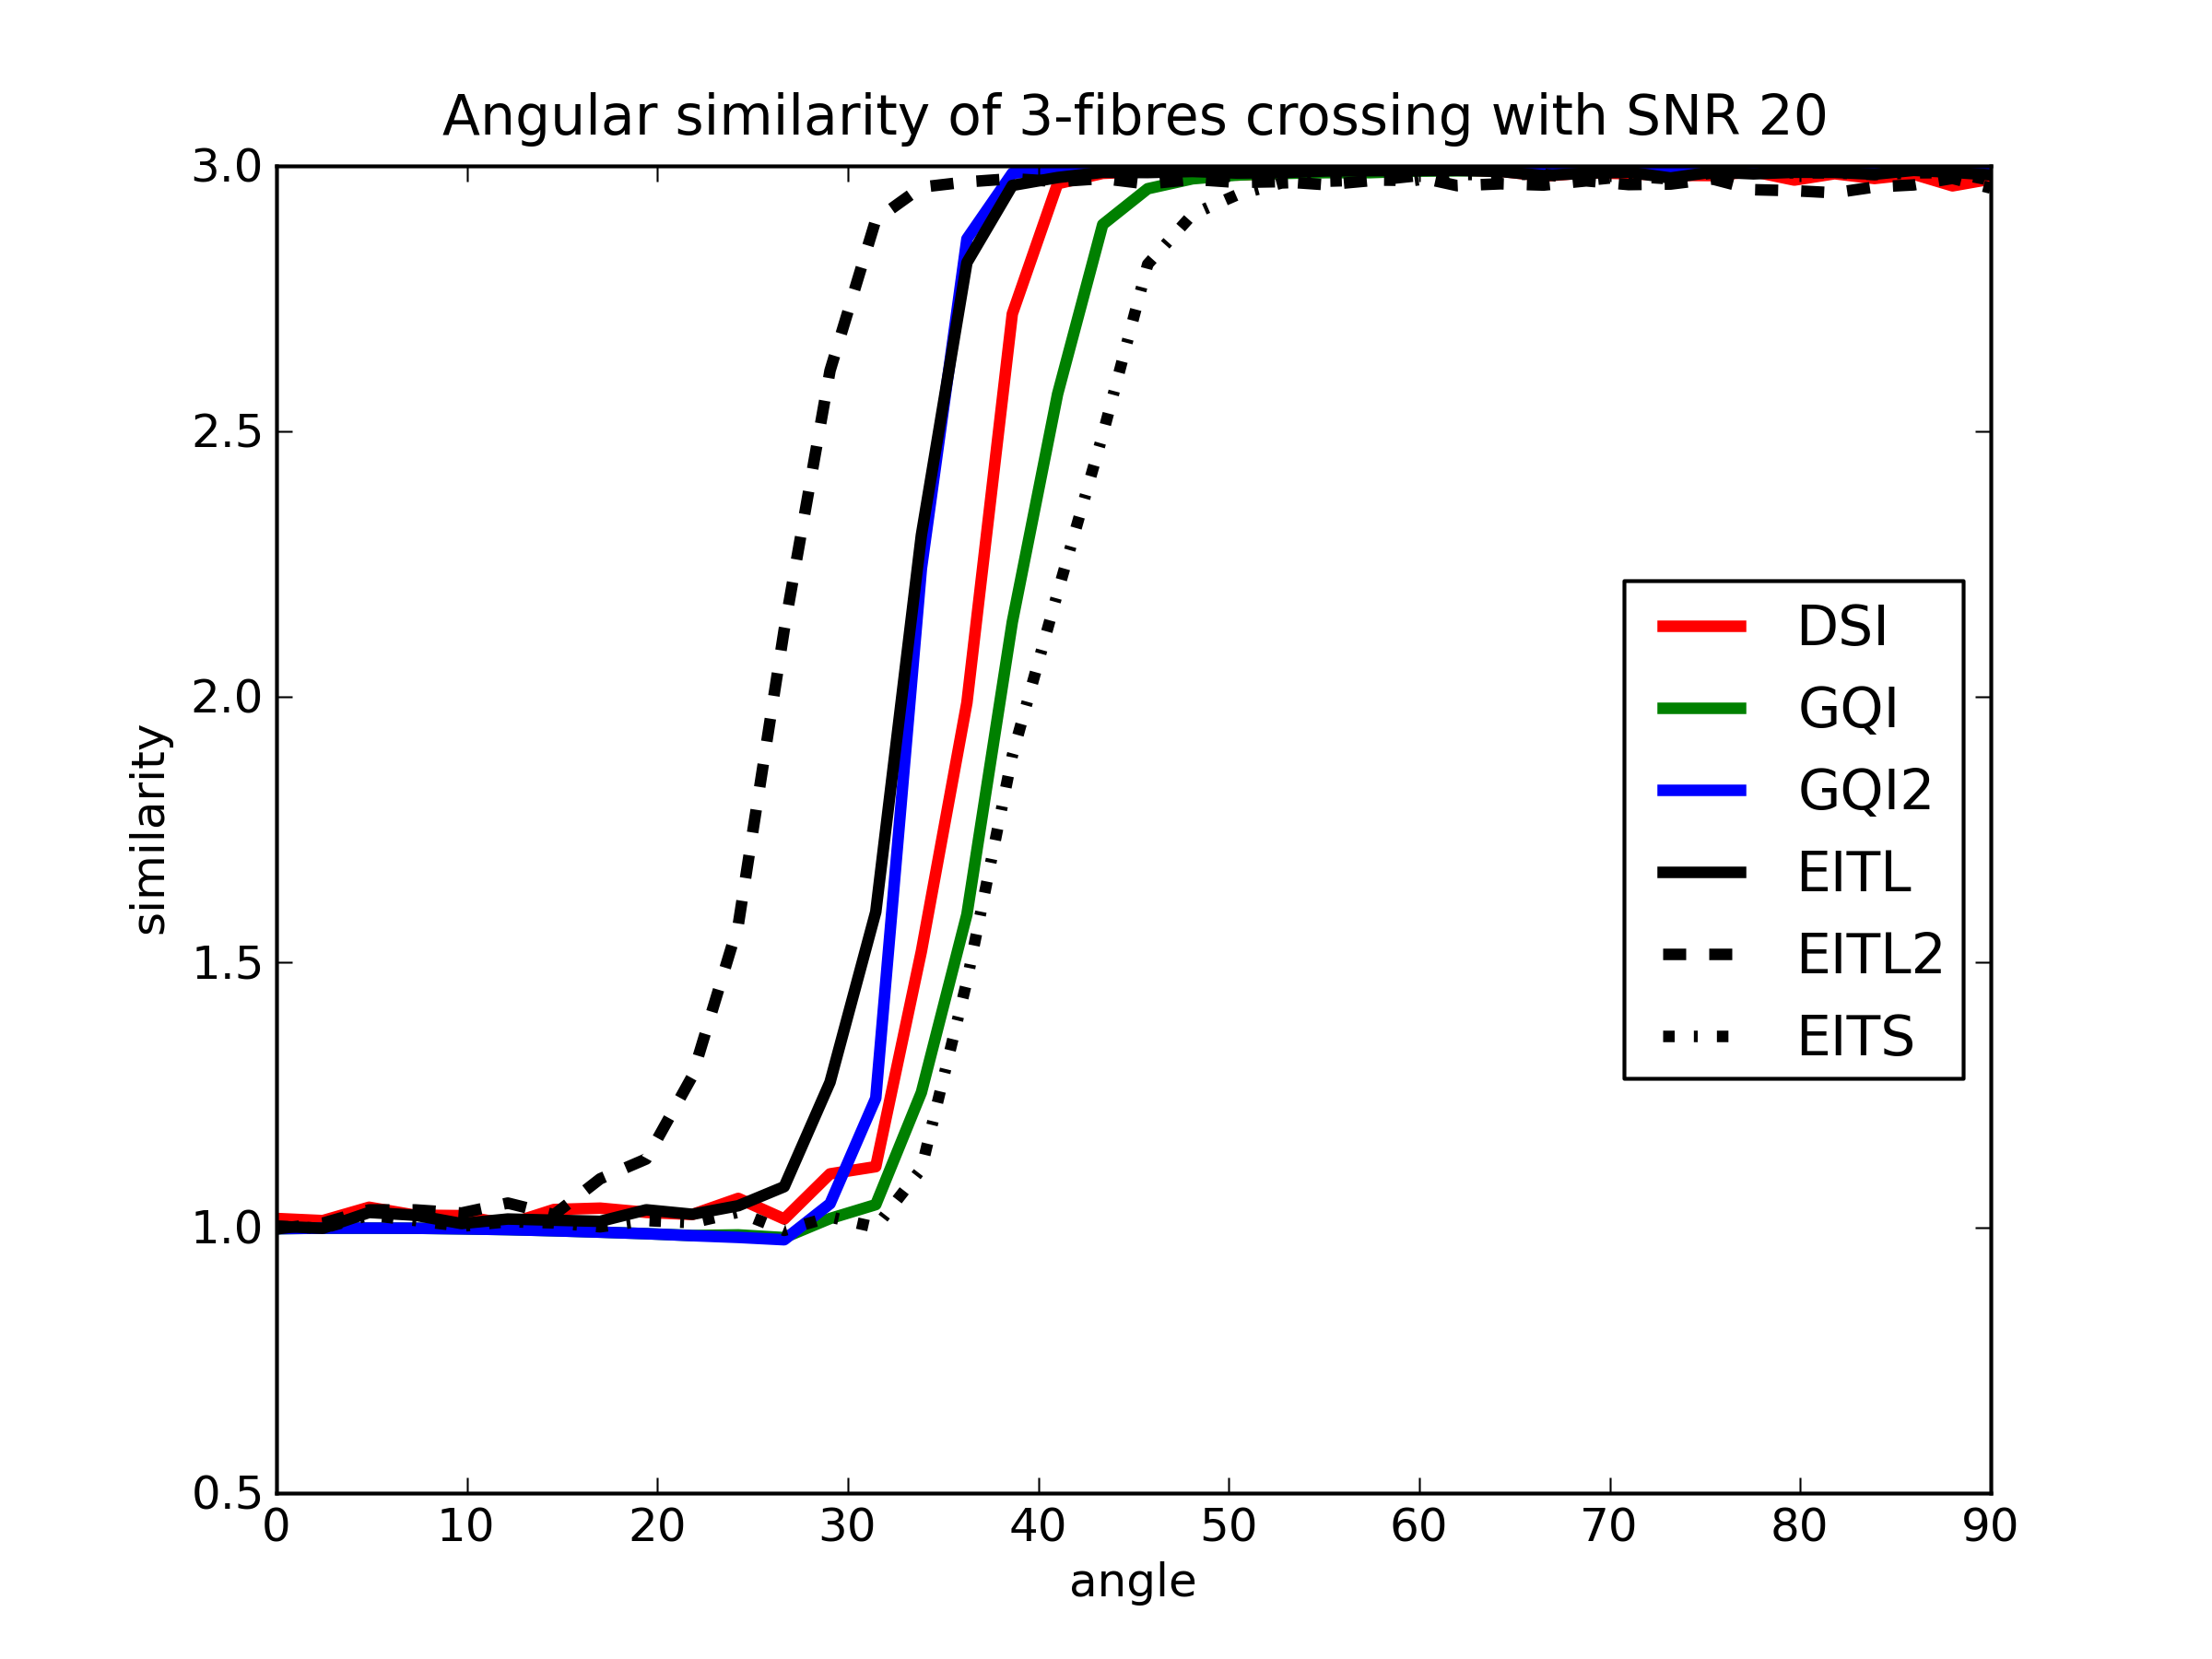
\includegraphics[scale=0.5]{last_figures/3_20}
\par\end{centering}

\caption{Average angular similarity of $3$-fibre crossings with SNR $20$.}


\label{Flo:3_20}
\end{figure}


These summarization plots give strong evidence that both DNI (EITL)
and in general EIT can be used to accurately generate spherical distribution
functions for the determination of the directional information of
the diffusion signal. They performed equivalently or better than the
current state-of-the-art grid-based reconstruction methods i.e DSI
and GQI. The determination of the fibre directions was not affected
considerably by noise. 

Furthermore, we can also see that GQI2 can do better than DSI, GQI
and that EITS gives results that are very similar to GQI. The parameters
used for these simulations were DSI: radial sampling $2.1-6$, hanning
filter width: $36$, GQI: $\text{\ensuremath{\lambda}=1.2}$, GQI2:
$\lambda=3$, and EITS, EITL, EITL2 were all calculated with the standard
options zonal width ($z=5^{\circ}$), grid size $17\times17\times17$,
radial sampling $0-5$ with $0.1$ steps and no further post-processing
or smoothing was used. All methods were using the same reconstruction
sphere with $642$ vertices and $1,280$ faces.

In these tests, EIT and fast EIT produced very similar results. For
example, a simple test for the $3$-fibre case as seen in Fig.~\ref{Flo:FastvsStandardEITL}
shows that there is close agreement between the two methods i.e.~their
results are nearly equivalent. We can therefore conclude that the
fast EIT is an acceptable approximation of the standard EIT.

%
\begin{figure}
\centering{}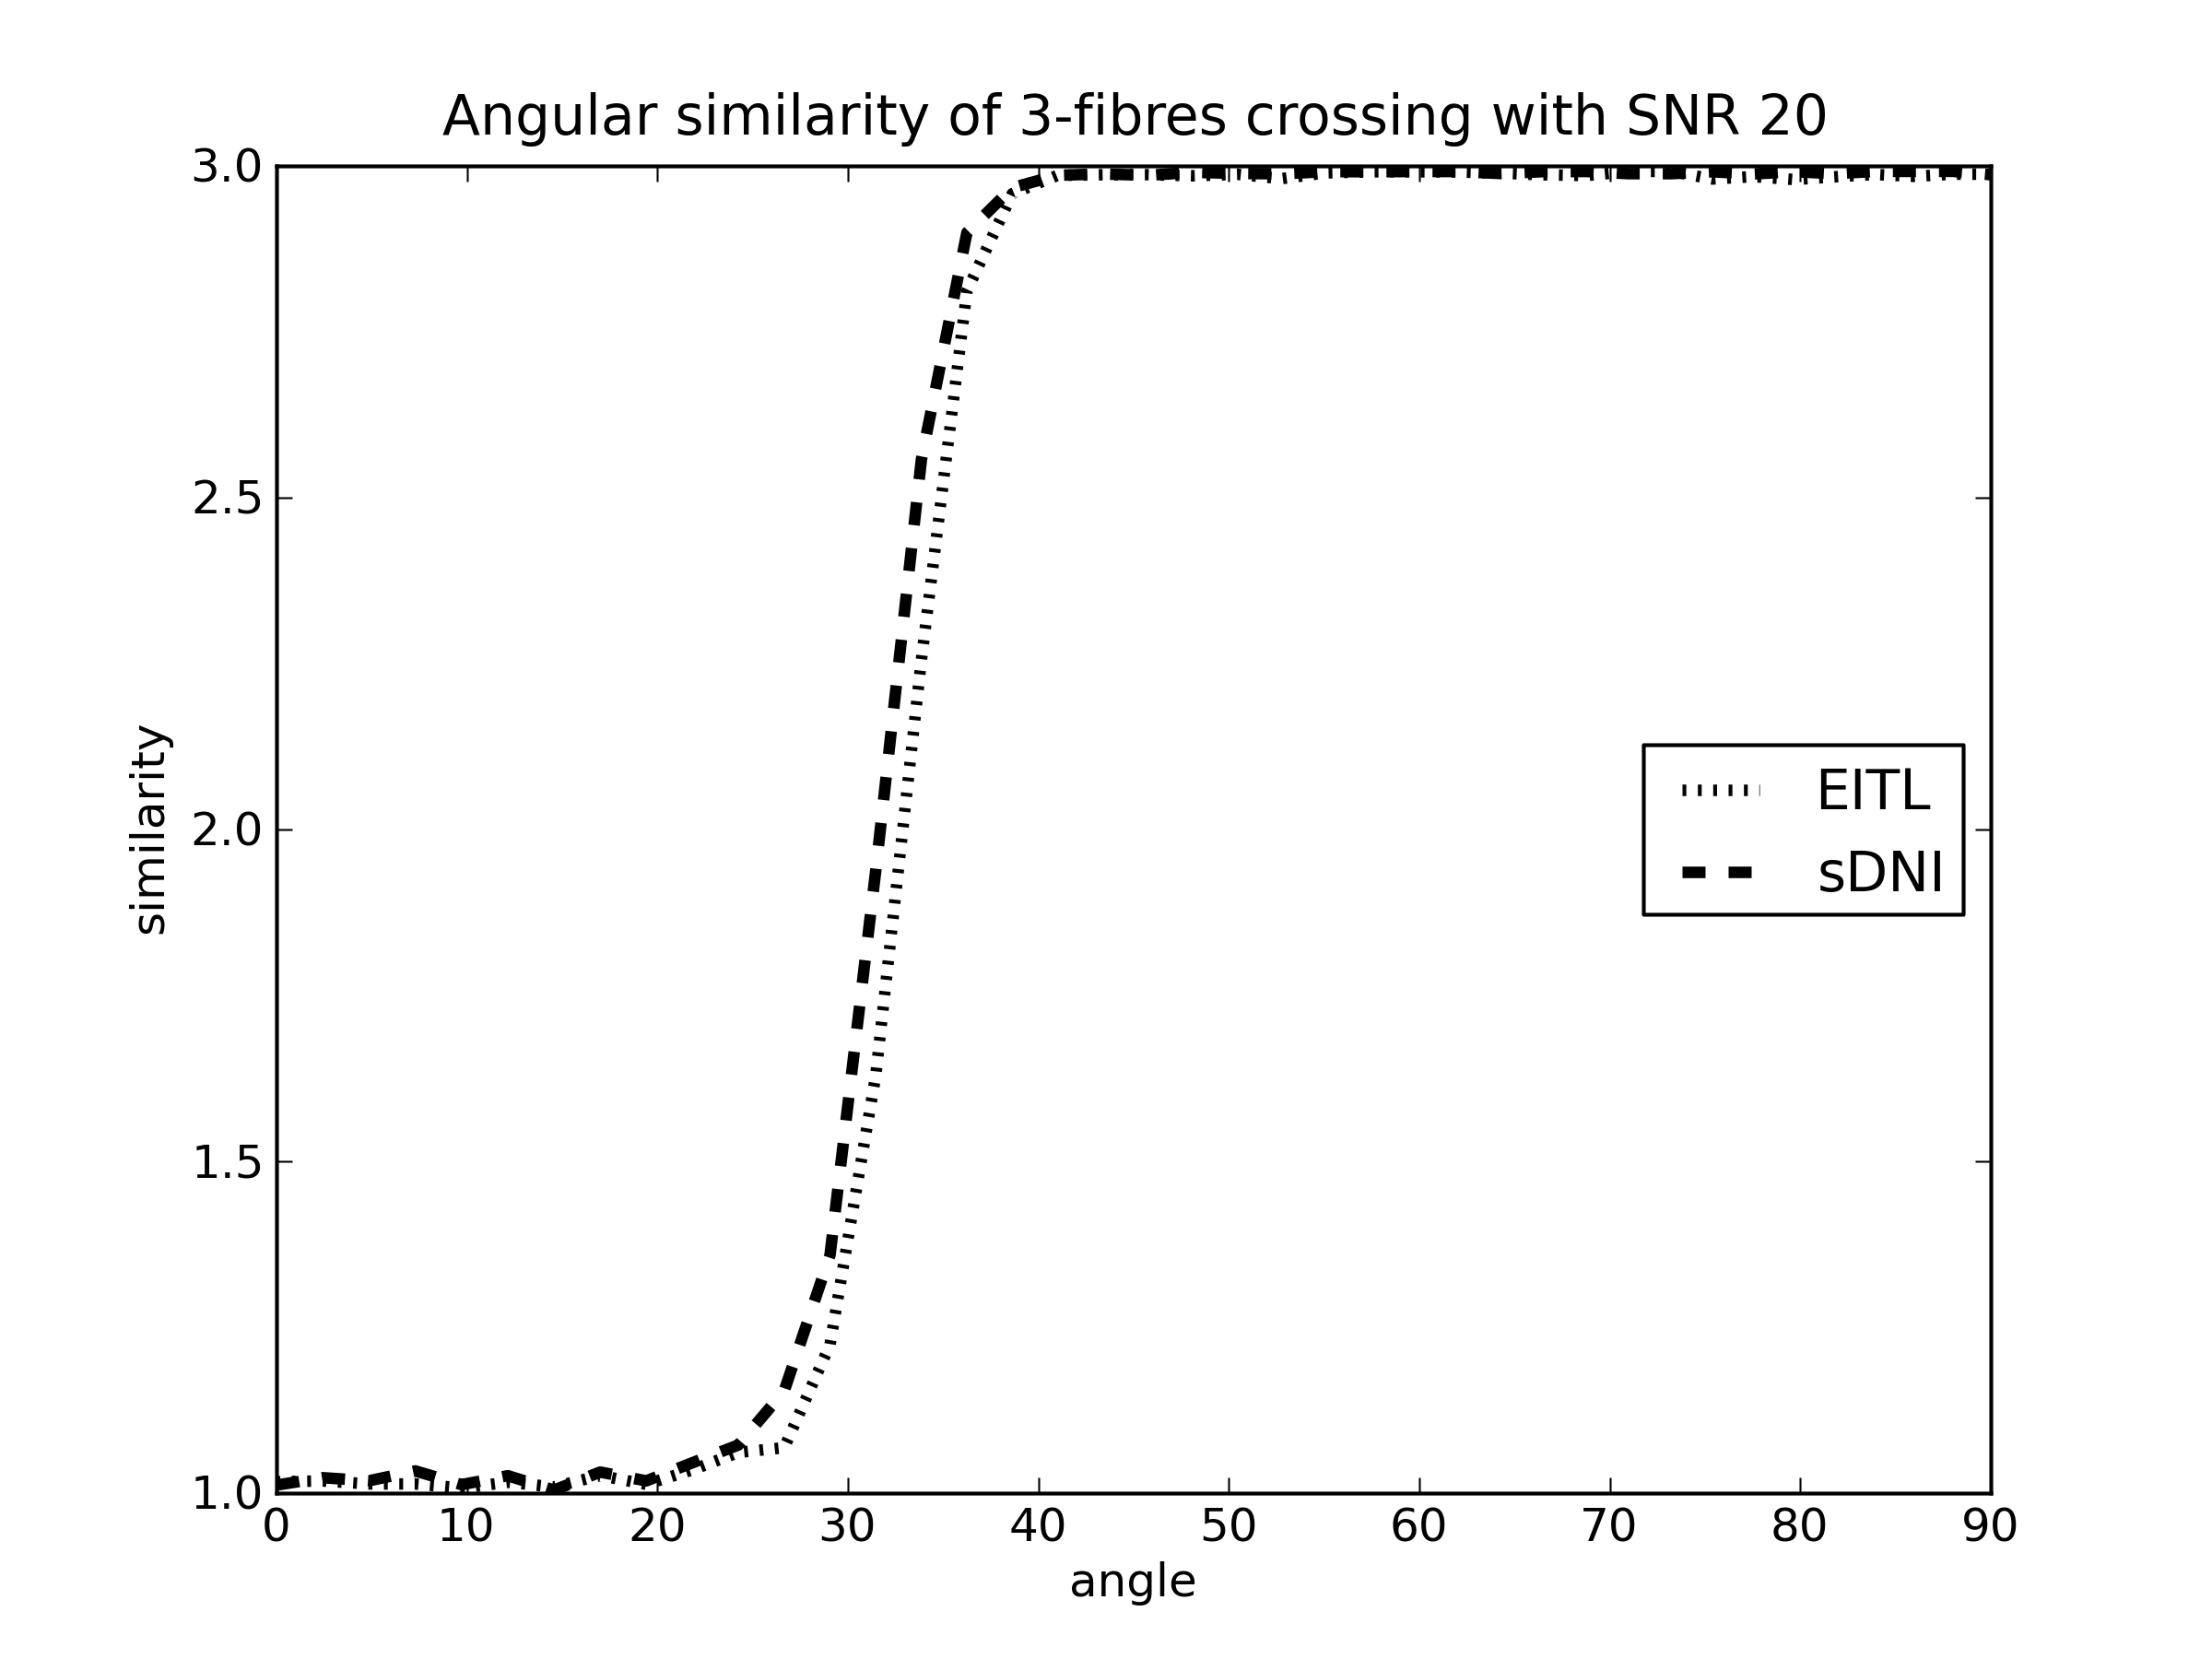
\includegraphics[scale=0.5]{last_figures/EITL_sEITL}\caption{This diagram shows that when we compute EITL with the fast or standard
method the results are nearly equivalent. The mean angular similarity
for the case of 3-fibres crossings is very similar when using standard
DNI or fast DNI (EITL). }
\label{Flo:FastvsStandardEITL}
\end{figure}



\subsubsection{Software Phantoms\label{sub:Digital-Phantoms}}

A software phantom generation tool was developed which can simulate
the diffusion weighted signal for one or more fibres represented by
different discrete 3D orbital functions. This work is an extension
of the phantom developed by Correia et al.~\cite{Correia2009} which
supported only paths with analytically calculated derivatives.

The idea here is that we first create any orbital function $f(t):\mathbb{R}\rightarrow\mathbb{R}^{3}$
and calculate numerically its derivatives at small steps $\Delta t$.
We can then scale it and centre it so that it fits in an image volume
of the desired size. We expect that many segments of the discrete
function $f$ will fall into every voxel in the volume and that more
curved parts of $f$ will have higher representation in the voxel
than less curved parts. For every segment, we can find the main direction
of the orbit $\mathbf{v}=\frac{f(t+1)-f(t)}{\Delta t}$ and calculate
the rotation matrix $\mathbf{R}$ that rotates $\hat{\mathbf{x}}=(1,0,0)$
to $\mathbf{v}$. Then, the signal for each element of the fibre for
a given b-value $b$ and a given gradient sampling direction $\hat{\mathbf{g}}$,
is given by the following Single Tensor formula

\begin{equation}
\Delta S=S_{0}\exp(-b\hat{\mathbf{g}}^{T}\mathbf{R}\bm{\Lambda}\mathbf{R}^{T}\hat{\mathbf{g}})\label{eq:step_signal}\end{equation}


\begin{flushleft}
where \foreignlanguage{british}{$S_{0}$ is the unattenuated signal
of the fibre, and the diffusion tensor is given by}
\par\end{flushleft}

\begin{center}
\begin{equation}
\bm{\Lambda}=\left(\begin{array}{ccc}
\lambda_{\parallel} & 0 & 0\\
0 & \lambda_{\perp} & 0\\
0 & 0 & \lambda_{\perp}\end{array}\right)\label{eq:step_tensor}\end{equation}

\par\end{center}

\noindent Therefore, the total signal of the voxel for one gradient
direction is given by the summations of all the contributions of the
$K$ elements in the voxel

\begin{equation}
S_{vox}=\sum_{i=1}^{K}\Delta S_{i}\label{eq:digital_phantom_signal}\end{equation}


In addition, we can generate simulations of more than one fibre by
generating a single volume for every orbit and then add them all together
to create complex configurations in the final volume. This is acceptable,
under the assumption that the diffusion is Gaussian in all compartments,
because the diffusion signal is additive i.e. the signal of a crossing
of two fibres is equal to the sum of the the signals of the individual
fibres. In this way, we can simulate phantoms with Multi Tensor based
diffusion signals as that described in Eq.~\ref{eq:multitensor}.
We can increase the thickness of the fibres using a typical smoothing
kernel or duplicate the fibres radially. At the end we can add different
levels of noise e.g. Rician or Gaussian noise with a prespecified
SNR. 

The method we use to create these software phantoms offers the opportunity
to simulate partial volume effects. If partial volume effects are
not desired, we need to normalize by dividing by the number of fibre
elements for each voxel. In Fig.~\ref{Flo:cool_phantoms} we can
see the volume renderings of two different phantoms created with the
method described here. This function is implemented in module $\texttt{dipy.sims.phantom}$.

%
\begin{figure}
\begin{centering}
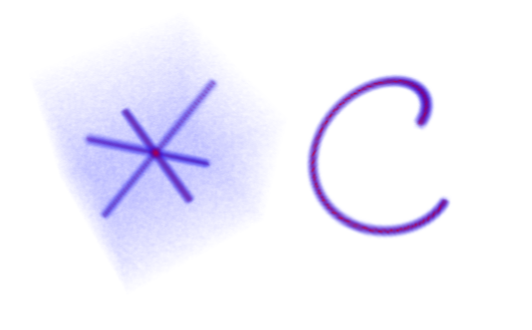
\includegraphics[scale=0.6]{last_figures/digital_phantom}
\par\end{centering}

\caption{Volume renderings of the unattenuated signals of two digital phantoms.
On the left 3 fibres intersect on regular angles with Rician noise
of SNR=$20$. On the right a helicoidal fibre is shown clear of noise.
For both phantoms $S_{0}=100$ and prolate tensors with eigenvalues
$\lambda_{\parallel}=1.4\cdot10^{-3}$ \foreignlanguage{british}{$m^{2}/sec$}
and $\lambda_{\perp}=.35\cdot10^{-3}m^{2}/sec$ were used.}


\centering{}\label{Flo:cool_phantoms}
\end{figure}



\subsubsection{Results with software phantoms}

With the purpose of comparing and visualizing the differences between
the reconstruction methods described in this chapter a phantom of
two crossing bundles was created. The bundles are crossing at an angle
of $90^{\circ}$. The phantom was generated using the method described
in the previous section. Here we describe the basic steps: (a) We
first represented the first bundle as a discrete straight path starting
from point $(-1,-1,0)$ and ending at point $(1,1,0)$ with using
$1,000$ time steps. (b) We scaled, centred and radially expanded
this path so that it fits a volume of size $64\times64\times64$.
This volume corresponds to the diffusion volume without any weighting.
(c) We then applied the weightings for all the following volumes corresponding
to non-zero b-values. (d) We replicated the same procedure for the
other bundle which initially started as an orbit from position $(-1,1,0)$
and ended at position $(1,-1,0)$. (e) We added the two volumes together
to create an 'x' shape (see Fig.~\ref{Flo:x-shape-thin-tensor},~\ref{Flo:x-shape-fat-tensor}).
(f) We added Rician noise with SNR=$5$. As in this chapter we concentrate
on Cartesian Lattice Q-space acquisitions we generated b-vectors and
b-values using a keyhole Cartesian sampling grid \cite{Tuch2002ThesisMIT}
with $515$ q-vectors. The maximum b-value was $11,538$ and the minimum
was $0$. Two sets of simulation experiments were performed each using
a Tensor of different shapes.

%
\begin{figure}
[th!]

\begin{centering}
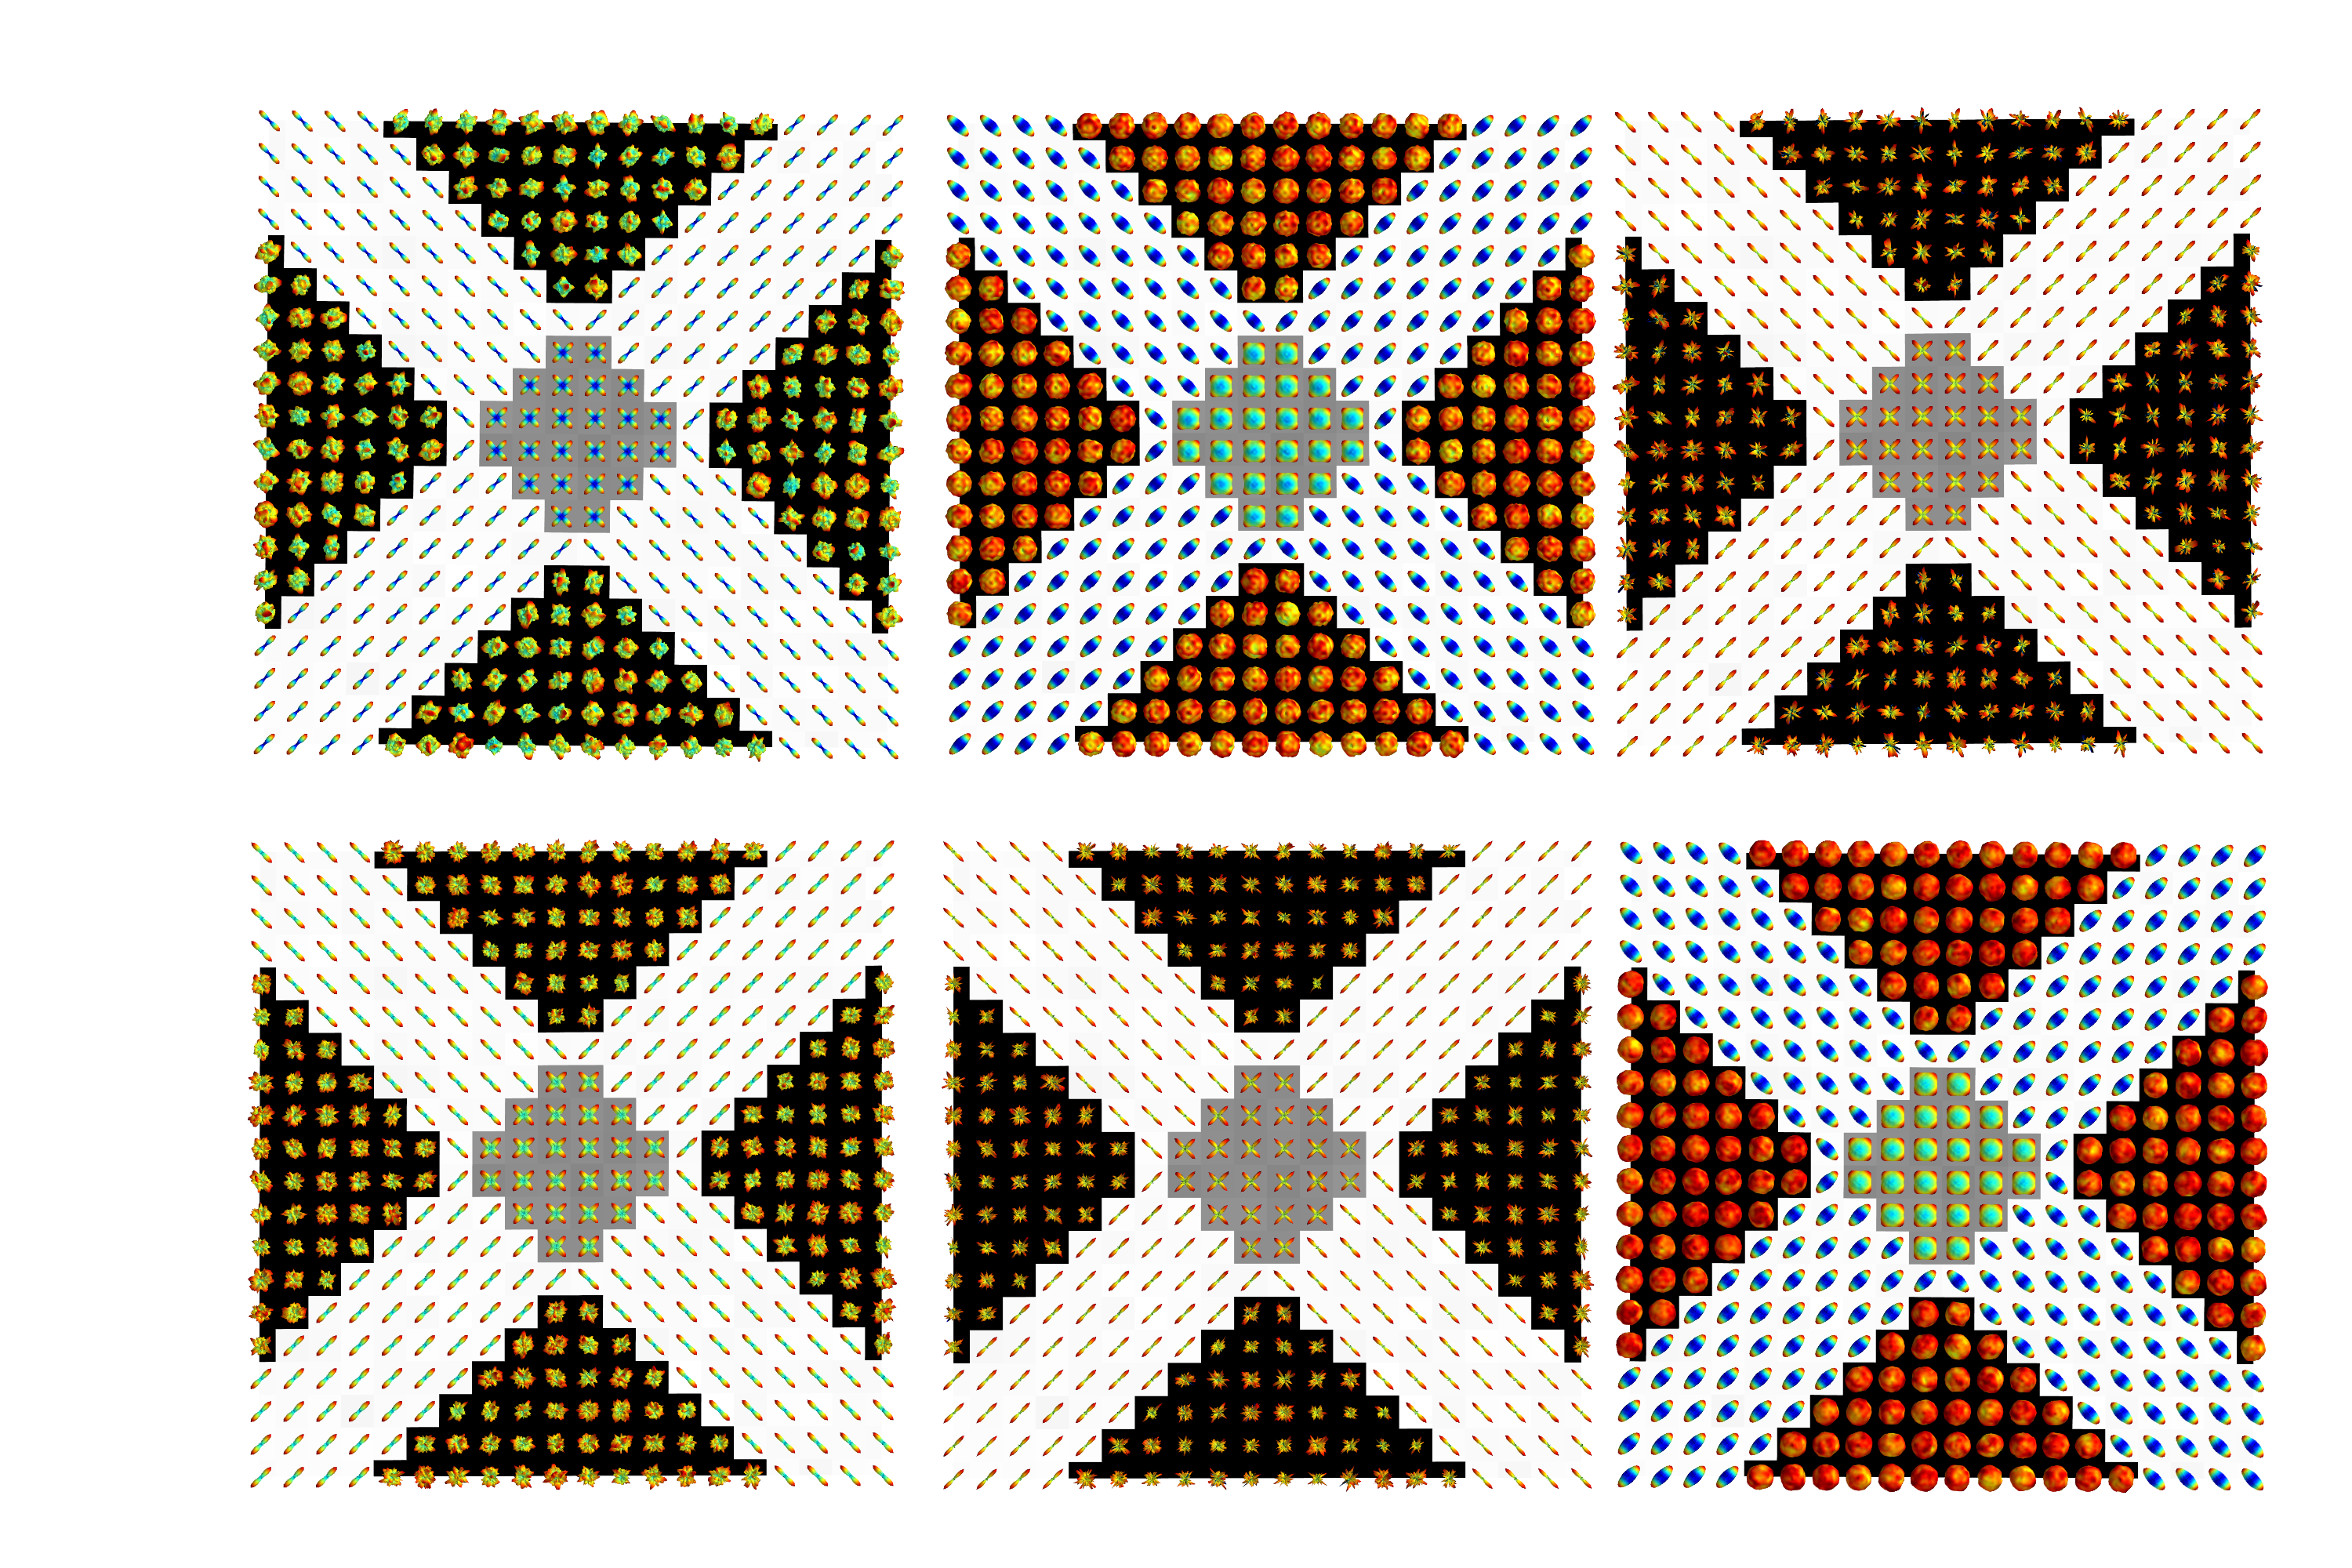
\includegraphics[scale=0.14]{last_figures/software_phantom_comparisons_rician_05}
\par\end{centering}

\caption{Results with an 'x' shape software phantom. Every single tensor compartment
had the following eigenvalues $\lambda_{\parallel}=1.4\times10^{-3}$
\foreignlanguage{british}{$\textrm{mm}^{2}/\textrm{sec}$} and $\lambda_{\perp}=0.1\times10^{-3}\textrm{mm}^{2}/\textrm{sec}$.
Rician noise was added with SNR = $5$. GQI is very similar to EITS,
GQI2 is very similar to EITL and DSI is very similar to EITL. In Fig.~\ref{Flo:x-shape-thin-tensor-zoomed}
the regions at the centers of the phantoms are depicted in higher
resolution.}


\centering{}\label{Flo:x-shape-thin-tensor}
\end{figure}


In the first experiment shown in Fig.~\ref{Flo:x-shape-thin-tensor},~\ref{Flo:x-shape-thin-tensor-zoomed}
we used a more anisotropic prolate tensor for the simulation with
eigenvalues $\lambda_{\parallel}=1.4\times10^{-3}$ \foreignlanguage{british}{$\textrm{mm}^{2}/\textrm{sec}$}
and $\lambda_{\perp}=0.1\times10^{-3}\textrm{mm}^{2}/\textrm{sec}$.
In the second experiment shown in Fig.~\ref{Flo:x-shape-fat-tensor}
and Fig.~\ref{Flo:x-shape-fat-tensor-zoomed} we used a much less
anisotropic prolate tensor with$\lambda_{\parallel}=1.7\times10^{-3}$
\foreignlanguage{british}{$\textrm{mm}^{2}/\textrm{sec}$} and $\lambda_{\perp}=0.3\times10^{-3}\textrm{mm}^{2}/\textrm{sec}$.
The values of $\lambda$ are based in \cite{Canales-Rodriguez2009}.
It is well known that noise has higher effect on less anisotropic
areas. We can see this effect by comparing the overlapped FAs of these
two two figures (\ref{Flo:x-shape-thin-tensor}, \ref{Flo:x-shape-fat-tensor}).
We can also see that all six methods (DSI, GQI, GQI2, EITL, EITL2,
EITS) can resolve correctly the fibre directions by looking at their
spherical distribution functions using a standard colour map. For
visualization purposes all ODFs are shown in relative size as they
have been scaled so that their maximum values correspond to $1$. 

Furthermore, we can easily observe that GQI is mostly similar to EITS,
GQI2 is very similar to EITL and DSI is mostly similar to EITL. The
fact that DSI ODFs are very similar to those of EITL ODFs is to be
expected as the two methods create theoretically the same real ODFs.
Remarkably, EITL can create these ODFs without using the Fourier Transform
neither using any filter or thresholds in r-space which are necessary
in DSI.

%
\begin{figure}
[ht!]

\begin{centering}
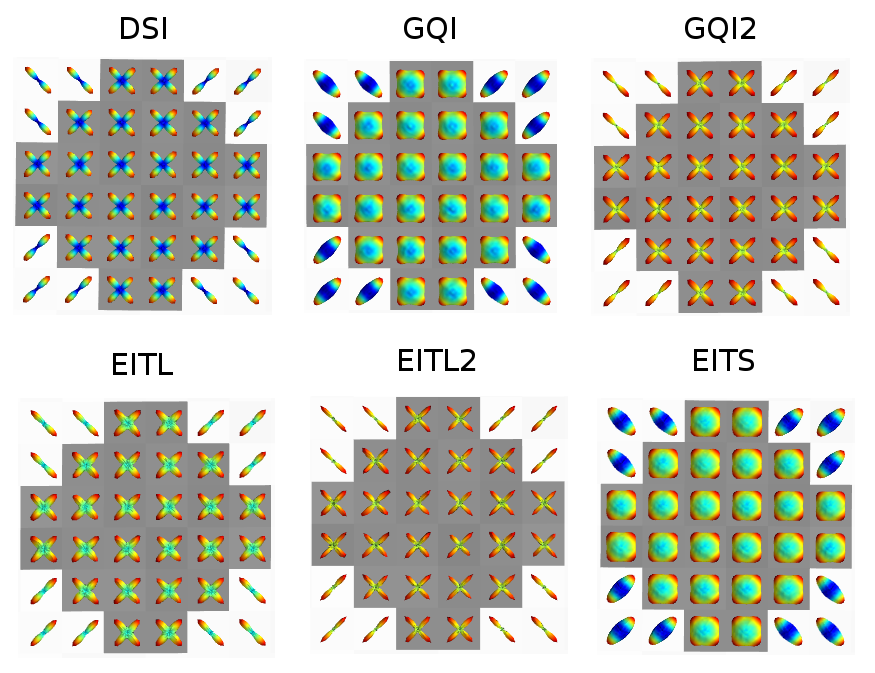
\includegraphics[scale=1.5]{last_figures/software_phantom_comparisons_rician_05_zoomed}
\par\end{centering}

\caption{Same as Fig.~\ref{Flo:x-shape-thin-tensor} showing in higher resolution
the spherical distributions in the centers of the phantoms.}


\centering{}\label{Flo:x-shape-thin-tensor-zoomed}
\end{figure}


%
\begin{figure}
[ht!]

\begin{centering}
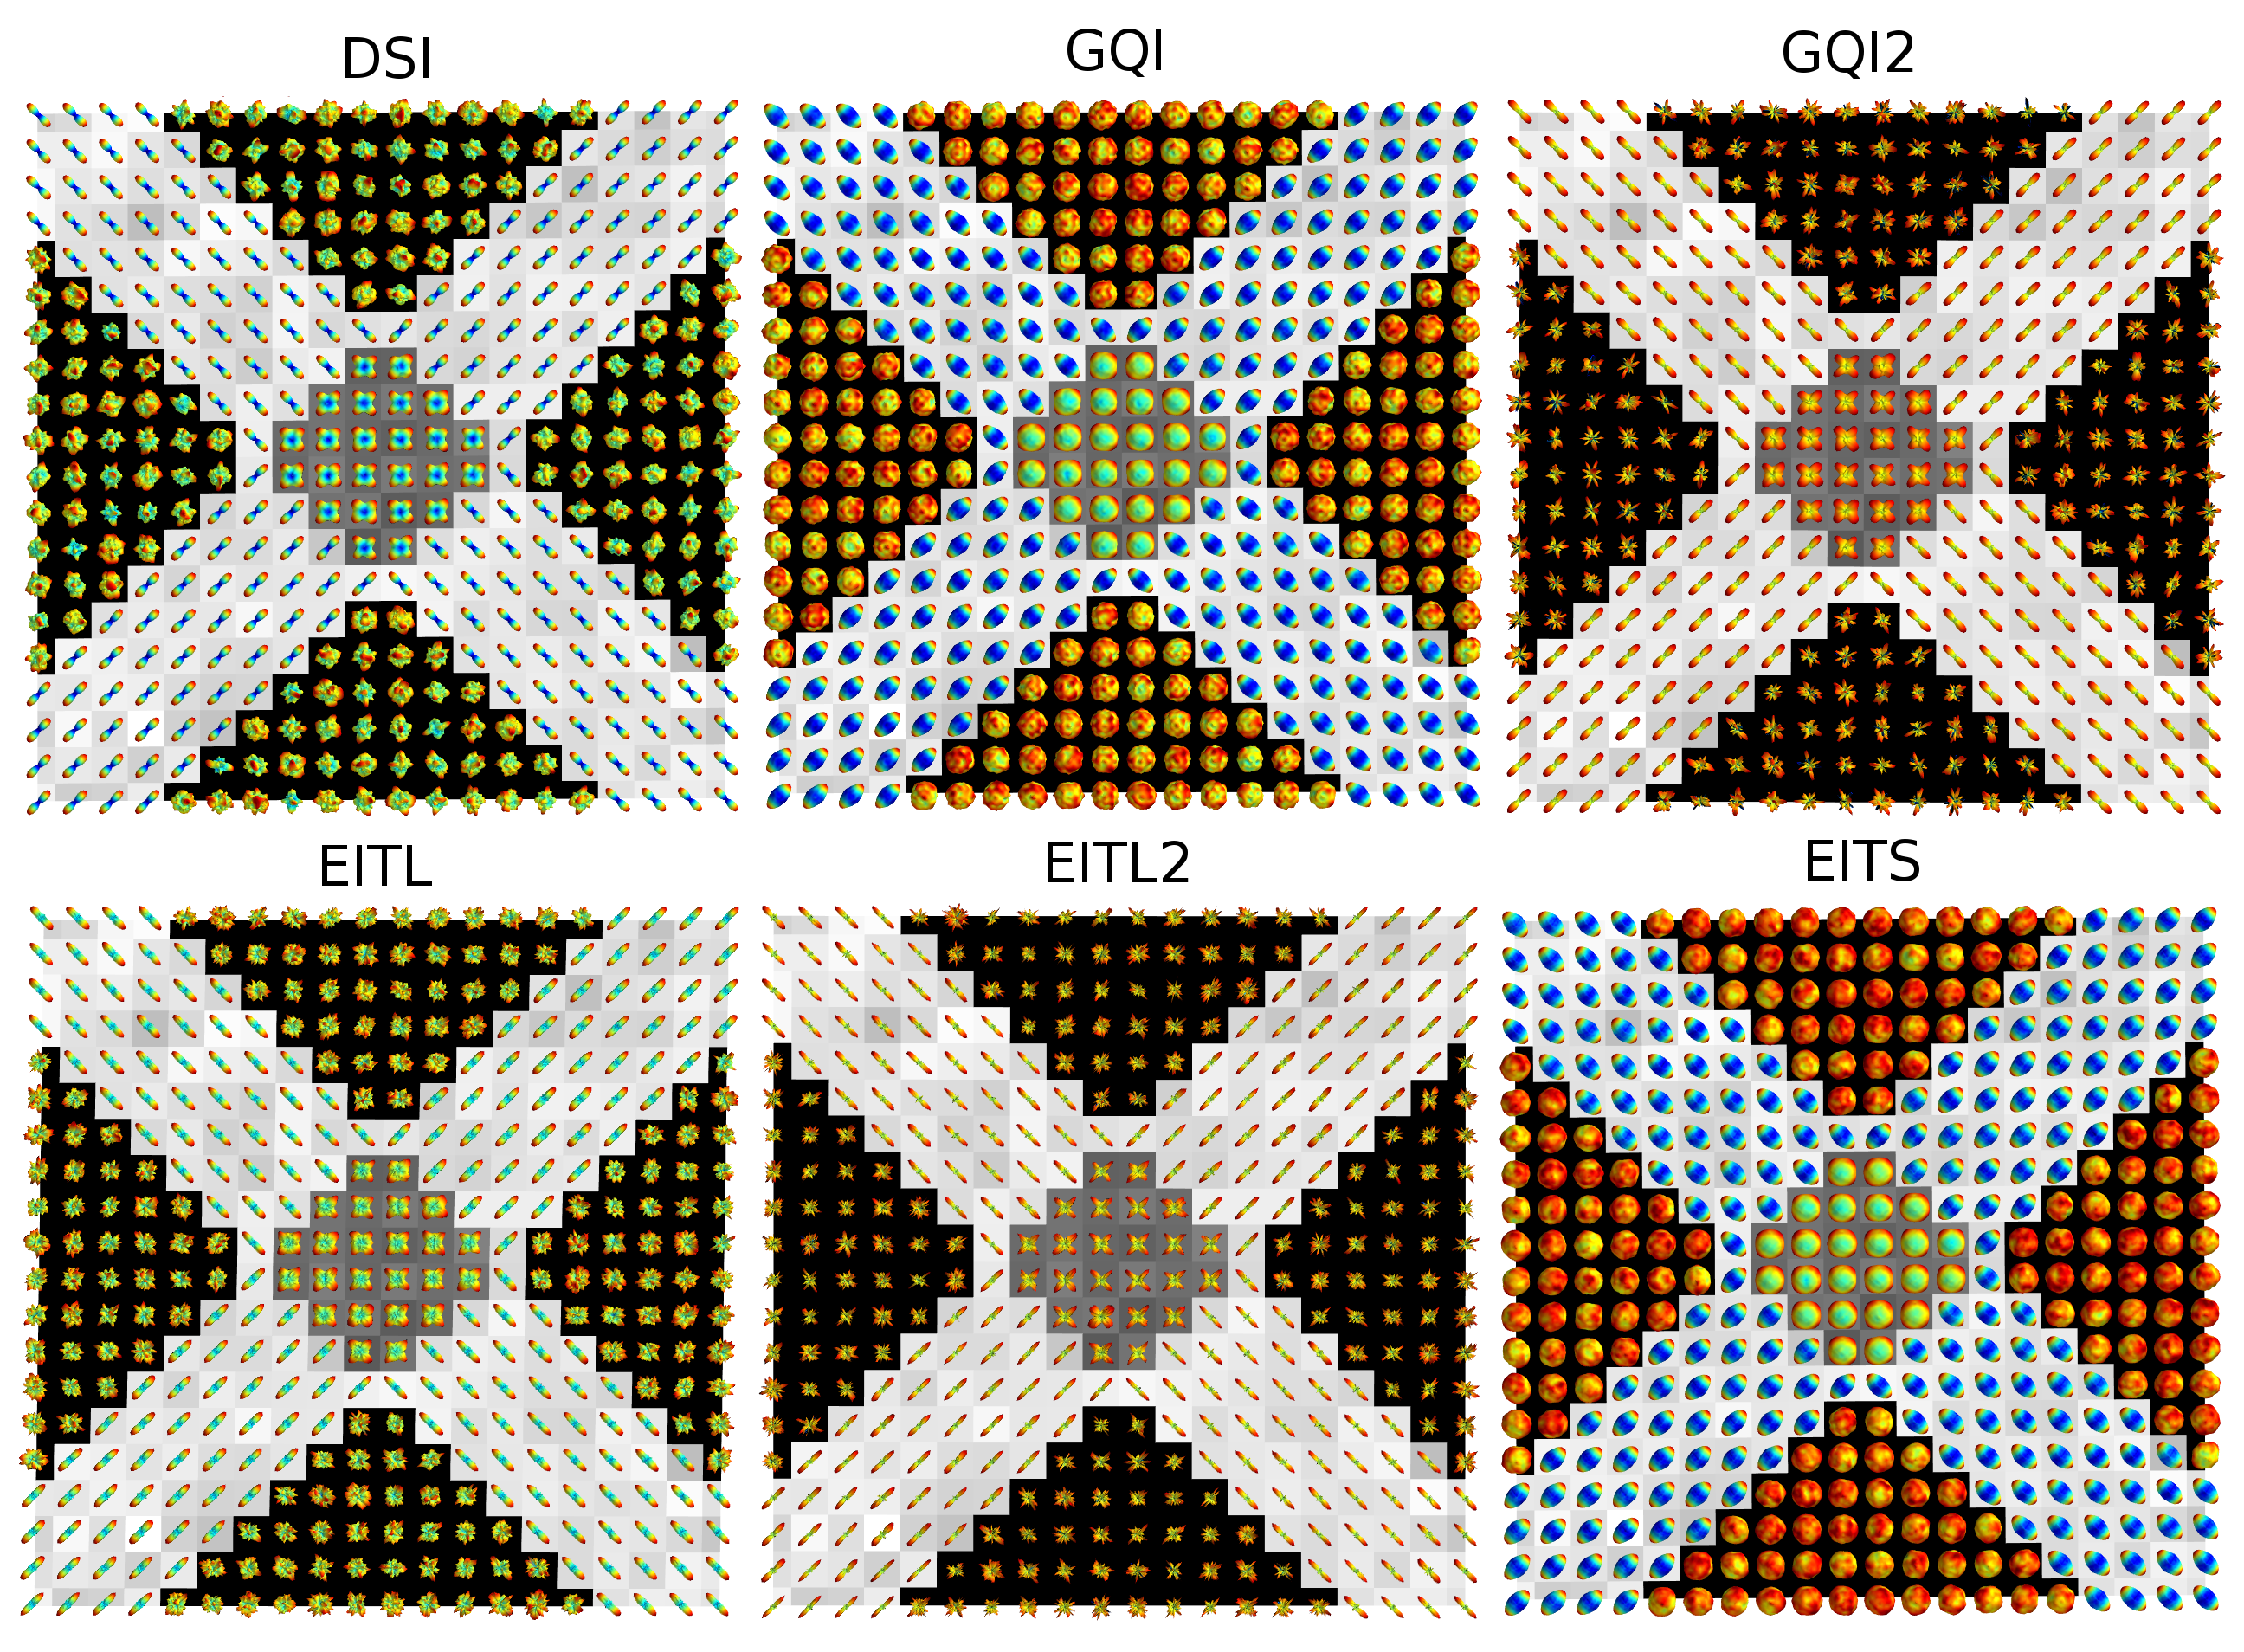
\includegraphics[scale=0.14]{last_figures/software_phantom_comparisons_rician_05_fat}
\par\end{centering}

\caption{Showing the spherical distribution functions (DSI, GQI, GQI2, EITL,
EITL2, EITS) of a software phantom generated by two bundles where
each bundle contains single tensors along the direction of the phantom.
On the crossing area, a dual Tensor effect in every voxel is observed.
Every single Tensor compartment had the following eigenvalues $\lambda_{\parallel}=1.7\times10^{-3}$
\foreignlanguage{british}{$\textrm{mm}^{2}/\textrm{sec}$} and $\lambda_{\perp}=0.3\times10^{-3}\textrm{mm}^{2}/\textrm{sec}$.
Rician noise was added with SNR=$5$. We also visualize simultaneously
the FA for this slice. We can see that in the crossing area (gray
background) the FA values drop considerably. However, the ODFs represent
precisely the crossing. }


\centering{}\label{Flo:x-shape-fat-tensor}
\end{figure}


Fig.~\ref{Flo:x-shape-thin-tensor}, \ref{Flo:x-shape-fat-tensor}
show that all the different grid-based reconstruction methods can
reconstruct correctly the underlying fibre directions even when noise
is present. However, we can see that when tensors are less anisotropic
the noise has a stronger effect in the resulting spherical distributions.
We can also see that GQI \& EITS are less sharp than DSI \& EITL and
these are less sharp than GQI2 \& EITL2. Also DSI, GQI2, EITL, EITL2
have much lower minima than GQI and EITS. 

%
\begin{figure}
[th]

\begin{centering}
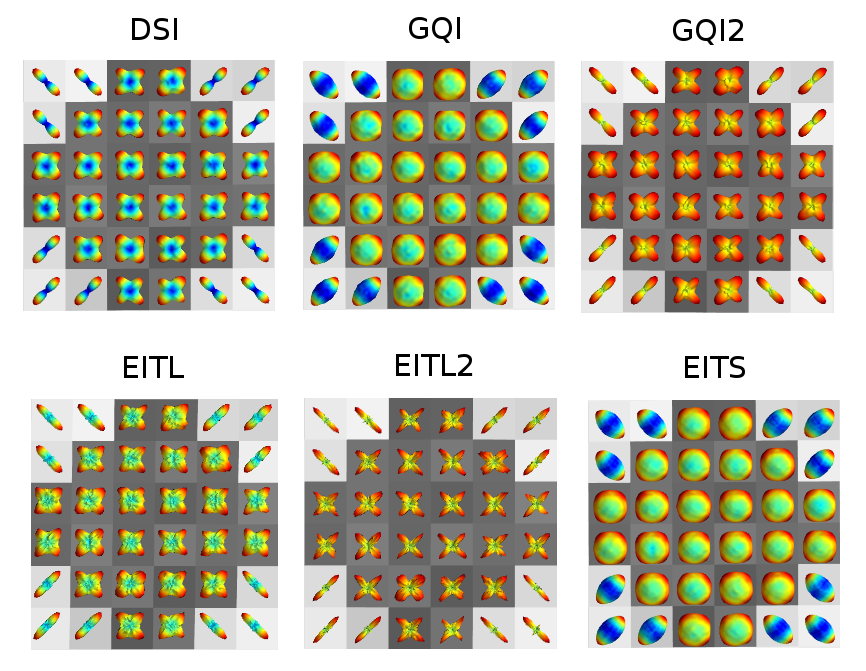
\includegraphics[scale=1.5]{last_figures/software_phantom_comparisons_rician_05_fat_zoomed}
\par\end{centering}

\caption{A zoomed version of Fig.~\ref{Flo:x-shape-fat-tensor} showing the
spherical distributions in the centers of the phantoms at higher resolution.}


\centering{}\label{Flo:x-shape-fat-tensor-zoomed}
\end{figure}


In the EIT-based reconstruction results shown in Fig.~\ref{Flo:x-shape-thin-tensor-zoomed}
and Fig.~\ref{Flo:x-shape-fat-tensor-zoomed} we do not use any amount
of smoothing as used in DSI (through hanning filter), GQI, GQI2 (through
sampling length) and it is extraordinary that we still obtain such
well defined distributions. If we want to apply some weighting/smoothing/denoising
in EIT-based methods that is simply possible through the spherical
angular smoothing approach described in section \ref{sub:Spherical-Angular-Smoothing}. 

The parameters used for these simulations were for DSI: radial sampling
$2.1-6$, hanning filter width: $36$ , GQI: $\text{\ensuremath{\lambda}=1.2}$,
GQI2: $\lambda=3$, and EITS, EITL, EITL2 were all calculated with
the standard options ($z=\pm5$) and no further post-processing or
smoothing was used. All methods were using the same reconstruction
sphere with $642$ vertices and $1,280$ faces.


\subsubsection{Results with humans}

We want to compare reconstruction methods on Cartesian grid-based
acquisitions first with data sets which are rich on directions and
commonly used for DSI processing. For this purpose we used a data
set which was available online at $\texttt{cmtk.org}$ from the Diffusion
Group at Ecole Polytechnique F�d�rale de Lausanne (EPFL), Switzerland.
So, this data set was obtained from a 3T scanner (TIM Trio, Siemens)
with a 32 channels head coil. The field of view was $210\times210\,\textrm{mm}^{2}$,
matrix size $96\times96$, and slice thickness $3\textrm{\,\textrm{mm}}$.
$44$ slices were acquired and the voxel resolution was $2.2\times2.2\times3.0\,\textrm{mm}^{3}$.
A $258$-point half grid acquisition scheme with a maximum b-value
of $8011\,\textrm{s}/\textrm{mm}^{2}$ also known as DSI515~\cite{Wedeen2008}
was used. The total acquisition time was $34\,\textrm{min}$ with
TR=$8200\,\textrm{ms}$ and TE=$165\,\textrm{ms}$.

%
\begin{figure}
[th!]

\begin{centering}
\includegraphics[scale=0.6]{last_figures/real_data_257_all_grid_methods_purple}
\par\end{centering}

\caption{Showing the same slice of a human brain reconstructed with 6 different
Cartesian grid q-space based methods. The ODFs are visualized on top
of the FA slice. A clearer presentation of a region near the left
upper corner (with purple shading) is given in Fig.~\ref{Flo:real_257_zoomed}
for all the $6$ methods.}


\centering{}\label{Flo:real_257}
\end{figure}


The parameters used for these simulations were for DSI: radial sampling
$2.1-6$, Hanning filter width: $36$, GQI: $\text{\ensuremath{\lambda}=1.2}$,
GQI2: $\lambda=3$, and for EITS, EITL, EITL2 were all calculated
using the standard options for zonal width ($z=5^{o}$) and spherical
angular smoothing ($s=0.05)$. All methods were using the same reconstruction
sphere $642$ vertices and $1,280$ faces. The results of this experiment
are shown on top of an FA slice of a healthy human in Fig.~\ref{Flo:real_257}
and in higher resolution in Fig.~\ref{Flo:real_257_zoomed}. It is
observed that EITL, EITL2 and EITS can be used for reconstructing
these data sets as their results appear very similar to the results
given by DSI, GQI and GQI2. We can also easily see that EITL and EITL2
are relatively sharp which can be of an advantage for the purpose
of recovering correctly the underlying real fibre directions.

%
\begin{figure}
[th!]

\begin{centering}
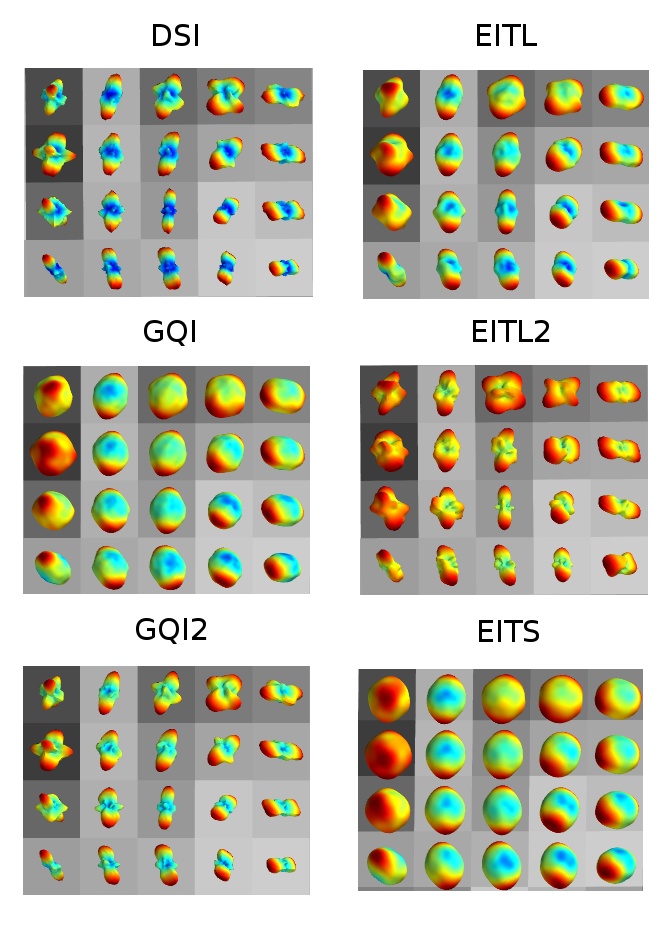
\includegraphics[scale=1.5]{last_figures/real_data_257_all_grid_methods_zoomed}
\par\end{centering}

\caption{The upper-left corners (purple shading region) of the panels of Fig.~\ref{Flo:real_257}
are shown here at higher resolution. These data sets belong to a real
human. In contrast with the results shown in simulations (see Fig.~\ref{Flo:x-shape-thin-tensor-zoomed})
we applied spherical angular smoothing with $s=0.05$ for EITL, EITL2
and EITS in order to remove small noisy spikes in the distributions.
In agreement with the results of Fig.~\ref{Flo:x-shape-thin-tensor-zoomed},
EITS is very similar to GQI. The difference between DSI, GQI2 and
EITL, EITL2 is smaller as a result of the application of angular weighting.}


\centering{}\label{Flo:real_257_zoomed}
\end{figure}


We also tested our results with another human brain data set generated
at a 3T scanner (TIM Trio, Siemens) at the Medical Research Council
Cognition and Brain Sciences Unit, Cambridge, UK. We used Siemens
advanced diffusion work-in-progress sequence, and STEAM \cite{merboldt1992diffusion,MAB04}
as the diffusion preparation method. The field of view was $240\times240\,\textrm{mm}^{2}$,
matrix size $96\times96$, and slice thickness $2.5\,\textrm{mm}$
(no gap). $55$ slices were acquired to achieve full brain coverage,
and the voxel resolution was $2.5\times2.5\times2.5\,\textrm{mm\ensuremath{{}^{3}}}$.
In this experiment a smaller number of gradient vectors were used.
A $102$-point half grid acquisition with a maximum b-value of $4,000\,\textrm{s}/\textrm{m\ensuremath{m^{2}}}$
was used. The total acquisition time was only $14\,\textrm{min}\,21\,\textrm{s}$
with TR=$8,200\,\textrm{ms}$ and TE=$69\,\textrm{ms}$.

%
\begin{figure}
[th!]

\begin{centering}
\includegraphics[scale=0.3]{last_figures/real_101_eitl_0\lyxdot 05}
\par\end{centering}

\caption{EITL ODFs rendered on top of FA of a human brain data set. A small
$102$-point half grid acquisition with a maximum b-value of $4,000\,\textrm{s}/\textrm{m\ensuremath{m^{2}}}$
was used. Fig.~\ref{Flo:real_101_CBU_left_up} and \ref{Flo:real_101_CBU_left_up_zoomed}
are zoomed versions of the same figure. We can see clearly single
fibres on the CC and CST areas but also crossing fibres at the Centrum
Semiovale and at the areas where big bundles cross. Also the non-white
matter areas are evidently more isotropic.}


\centering{}\label{Flo:real_101_CBU}
\end{figure}


%
\begin{figure}
[th!]

\begin{centering}
\includegraphics[scale=0.8]{last_figures/real_101_eitl_0\lyxdot 05_left_up_purple}
\par\end{centering}

\caption{The upper part of Fig.~\ref{Flo:real_101_CBU} is shown here at higher
resolution. The purple shaded part is given in higher resolution in
Fig.~\ref{Flo:real_101_CBU_left_up_zoomed}}


\centering{}\label{Flo:real_101_CBU_left_up}
\end{figure}


%
\begin{figure}
[th!]

\begin{centering}
\includegraphics[scale=1.5]{last_figures/real_101_eitl_0\lyxdot 05_left_up_zoomed}
\par\end{centering}

\caption{EITL ODFs of 1-fibre, 2-fibre and 3-fibre crossings from a real human
data set of $101$ applied weighted diffusion volume and $1$ without
weighting $(b0)$ . This picture is a zoomed version of the purple
shaded area shown in Fig. \ref{Flo:real_101_CBU_left_up}.}


\centering{}\label{Flo:real_101_CBU_left_up_zoomed}
\end{figure}


In Fig.~\ref{Flo:real_101_CBU} a slice is shown where different
parts of white matter are visible with the FA background image. We
can clearly see structures like the Corpus Callosum (CC) and Cortical-Spinal
Tract (CST) and Centrum Semiovale areas. The ODFs of EITL are shown
superimposed on the FA. The parameters used for EITL were: a standard
zonal width $z=5^{\circ}$ and spherical angular smoothing $s=0.05$
with the same reconstruction sphere ($642$ vertices, $1,280$ faces)
as before.

For illustration purposes the upper part of Fig.~\ref{Flo:real_101_CBU}
is depicted again in Fig.~\ref{Flo:real_101_CBU_left_up}, and the
region with purple shading from Fig.~\ref{Flo:real_101_CBU_left_up}
is given at an even higher resolution in Fig.~\ref{Flo:real_101_CBU_left_up_zoomed}.
We used Mayavi \cite{ramachandran2011mayavi}, a Python visualization
library based on VTK to make the visualizations shown in the figures
of this section.

Although less directions were used in this acquisition scheme we obtain
a similarly accurate depiction of the underlying white matter structure
in comparison with that of $258$ directions. This gives great hope
that we can use grid-based reconstruction methods with half-grid sequences
with $~100$ gradient directions. This was also shown by \cite{Kuo}
and \cite{Yeh2010} who used similar number of directions. 

In all the figures with real data sets we can see single fibres as
those usually found at the center of CC, and $2$ or $3$-fibre crossings
in the intersection areas of CC with the CST and other bundles. 

We can see for example in Fig.~\ref{Flo:real_101_CBU_left_up_zoomed}
that the effect of spherical angular smoothing can help alleviate
the noise effects and focus our concentration on depicting the major
directions which are also of highest concern. 


\subsection{Anisotropy metrics}

Until this moment we discussed about density functions on the sphere
as a way to represent complex fibre directionality in the voxel. These
density functions are represented as multidimensional vectors containing
$200$ or more dimensions in each voxel and it can be cumbersome to
use them directly for subject comparisons or visualization purposes.
For this purpose most people use simple scalar summarizing metrics
e.g. Tensor-based FA, MD or ODF-based such as the Generalized FA (GFA)
\cite{Tuch2002}. In this section we will show that a similar scalar
function like FA can be constructed non-parametrically. We call this
NPA which stands for non-parametric anisotropy. We will also start
experimenting with metrics that have more than one scalar value and
can represent more accurately the directionality in each voxel that
is lost with FA, GFA and MD. We will investigate and explain here
the realms and robustness of Quantitative Anisotropy which was first
introduced by Yeh et al. \cite{Yeh2010}.


\subsubsection{Non-parametric Anisotropy}

Local voxelwise measures such as fractional anisotropy (FA), apparent
diffusivity coefficient (ADC), or mean diffusivity (MD) have been
extensively adopted in clinical and applied research practice based
on diffusion weighted MR imaging (dMRI). This underlines the need
for valid and reliable measures which can indicate the degree of local
organisation of white matter in the brain. The measures listed above
are based on the parametric simple diffusion tensor (SDT or DTI) model
\cite{Basser1994} which works well when there is a single dominant
fibre direction. When the local organization is more complex however,
the information it provides is not so valid \cite{Yeh2010,Tuch2002ThesisMIT}.
We show how model-free, alternatives can yield non-parametric anisotropy
(NPA). These are constructed from the GQI ODF. We apply exact analytical
results which show the form of the GQI-ODF when the single tensor
model is correct, and further indicate how the tensor's parameters
may be estimated from this model-free approach. We compare the performance
of these parametric and non-parametric measures for simulated data.

Simulations were computed for a $102$-point grid sampling scheme,
with a maximum b-value of $4,000\,\textrm{s}/\textrm{mm}^{2}$. The
simulated fibre was aligned with the gradient frame of reference,
and the diagonal elements of the diffusion tensor, D, where chosen
to match typical values for white matter: $\lambda_{1}=1.4\times10^{-3}$
$\textrm{mm}^{2}/\textrm{s}$, and $\lambda_{2}=\lambda_{3}=0.35\times10^{-3}$
$\textrm{mm}^{2}/\textrm{s}$. Variable fibre orientation was realised
by spatially rotating the simulated fibres at discrete orientations.
$100$ orientations were used, which spanned uniformly the space of
$(\theta,\phi)$. 

In addition to the SDT a two compartment model with an isotropic component
was added with volume fraction $0.5$ and diffusivity $0.7\times10^{-3}$
\foreignlanguage{british}{\textbackslash{}textrm\{mm\}\textasciicircum{}\{2\}/\textbackslash{}textrm\{s\}}.
For each acquisition scheme and fibre type, the \textquotedblleft{}ideal\textquotedblright{}
(noise-free) diffusion weighted signals were calculated according
to the SDT model, assuming a constant ideal value of the baseline
signal $S_{0}=100$. Complex Gaussian noise was then superimposed
upon the ideal signals to provide the complex noise-contaminated signals
and their magnitude was then obtained. This results in noisy values
with a Rician distribution, which can be scaled in order to set the
signal to noise ratio to any desired level. In this study the SNRs
were $20$, $40$, $60$, $80$ and $100$. The GQI ODF and SDT were
fitted using $\texttt{DIPY}$ ($\texttt{dipy.org}$). 

The GQI ODF was calculated for a tessellated spherical icosahedron
with $362$ vertices and $720$ faces. Two values ($1.2$ and $3.5$)
were used for $\lambda$, the diffusion sampling length. Non-parametric
FA, NPA, was calculated from the ODF by: 
\begin{enumerate}
\item Locating the vertex $V_{1}$ with maximum GQI ODF value $\mathrm{max}_{1}$.
\item With $V_{1}$ as pole, locating the vertex $V_{2}$ on the corresponding
equatorial band of width \textpm{}5 degrees with maximum GQI ODF value
$\textrm{max}_{2}$.
\item Locating a vertex $V_{3}$ in the equatorial band at approximately
$90$ degrees away from $V_{2}$, denoting the GQI ODF value of $\textrm{max}_{3}$
at $V_{3}$. 
\item With $\textrm{npd}_{1}=\textrm{max}_{1}^{2}$, $\textrm{npd}_{2}=\textrm{max}_{2}^{2}$,
and $\textrm{npd}_{3}=\textrm{max}_{3}^{2}$, non-parametric anisotropy
(NPA) was calculated by applying the classical FA formula \ref{eq:FA_classical}
to the 3 values ($\textrm{npd}_{1},\textrm{\,\ npd}_{2},\,\textrm{npd}_{3}$). 
\end{enumerate}
The rationale for the squared ODF values is based on Tuch's formula
(Eq.~\ref{eq:tuchs_gaussian_odf}) for the ODF in the SDT case which
implies that the ODF in the $3$ principal axes directions of the
tensor is proportional to the square root of the corresponding eigenvalue
of the tensor. We have further derived an exact formula (see section~\ref{sub:Tensor-in-GQI}):
$\mathrm{max_{j}}\propto\sqrt{\lambda_{j}}\,[\Phi(cL_{\Delta}/\sqrt{\lambda_{j}})-.5]$
where $c$ is a constant that depends on the acquisition parameters,
and $\Phi$ is the cumulative distribution function of the standard
Gaussian distribution. 

The average NPA and FA are presented in Fig.~\ref{Flo:NPA_1} and
\ref{Flo:NPA_2} for $200$ simulations for each noise level, and
single fibres with or without an isotro- pic component and with different
diffusion sampling length. We can see that NPA gives very similar
results with FA and as expected it is modulated by the degree of smoothing
controlled by the value of the diffusion sampling length. 

We plan to extend this approach with voxels containing multiple peaks
where FA would be unable to give an informative result and also extend
it to other types of ODFs. In summary, we have shown that an informative
new scalar anisotropy function (NPA) can be calculated without fitting
just from the GQI ODF which promises to be a model-free proxy for
FA. NPA differs from GFA \cite{Tuch2004} in that it uses just $3$
values of the GQI ODF with a geometric relationship instead of the
entire ODF. 

%
\begin{figure}
[th!]

\begin{centering}
\includegraphics[scale=0.7]{figures/NPA_L_Delta1\lyxdot 2}
\par\end{centering}

\caption{Comparison of NPA with FA for single fiber with and without an isotropic
compartment at a range of signal to noise ratios.}


\label{Flo:NPA_1}
\end{figure}


%
\begin{figure}
[th!]

\begin{centering}
\includegraphics[scale=0.7]{figures/NPA_L_Delta3\lyxdot 5}
\par\end{centering}

\caption{As in Fig.~\ref{Flo:NPA_1} but with higher diffusion sampling length
- less smoothing.}


\label{Flo:NPA_2}
\end{figure}



\subsubsection{Quantitative Anisotropy\label{sub:Quantitative-Anisotropy}}

Quantitative anisotropy (QA) was first used by Yeh et al.~\cite{Yeh2010}
as a way of representing the peaks of the ODF with as few values as
possible. This works in the following way: a) we create the ODF, b)
we find the peaks using Alg. \ref{Alg:PeakFinding}, c) then $QA_{i}$
is equal to the peak $i$ minus the minimum value for the entire ODF.
This is illustrated in Fig.~\ref{Flo:QA_sketch} where we can see
a star-shaped ODF with three peaks (symmetric) ($PK$). This ODF can
be represented just with $3$ QA values where for example the highest
value will be: $QA_{0}=\max(\bm{\psi}_{GQI})-\min(\bm{\psi}_{GQI})$,
where $\max(\bm{\psi}_{GQI})$ is the value of the first peak $PK_{0}$,
and $QA_{2}=PK_{2}-\min(\bm{\psi}_{GQI})$ with $PK_{0}\geq PK_{1}\geq PK_{2}$.

%
\begin{figure}
[th!]

\begin{centering}
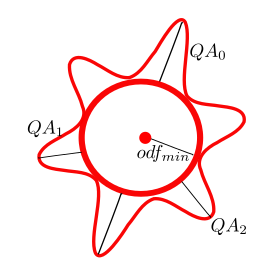
\includegraphics[scale=0.6]{QA}
\par\end{centering}

\caption{QA is calculated from an ODF. The sphere represents the {}``isotropic''
component (minimum value) of a GQI ODF (star) which will be removed
from the calculation of QA. QA acts like a differential component
with higher values in anisotropic areas and lower in isotropic. The
big advantage over FA is that it can represent crossings.}


\label{Flo:QA_sketch}
\end{figure}


QA acts like a differential operator which is higher on anisotropic
ODFs and lower on more isotropic. Actually, for a purely isotropic
ODF, $QA=\bm{0}$. QA can be also easily normalized by the maximum
ODF value of all voxels which is usually at the CSF where there is
a great amount of water. If this normalization is in effect then we
can very easily remove the background noise i.e. non-white matter
areas, scalp, skin, muscles etc. just because these will have very
low QA values. We can see this interesting property of QA in Fig.~\ref{Flo:QA_directions}.
Of course the most important property of QA is that it can resolve
crossings and assign a weight for every peak. We will make great use
of these weightings in Chapter 3. for the creation of tractographies.
Fig.~\ref{Flo:QA_directions} was created using DSI Studio %
\footnote{$\texttt{dsi-studio.labsolver.org}$%
} and the sequence parametrization is the same with the one provided
in the experiments of the next section.

%
\begin{figure}
[th!]

\begin{centering}
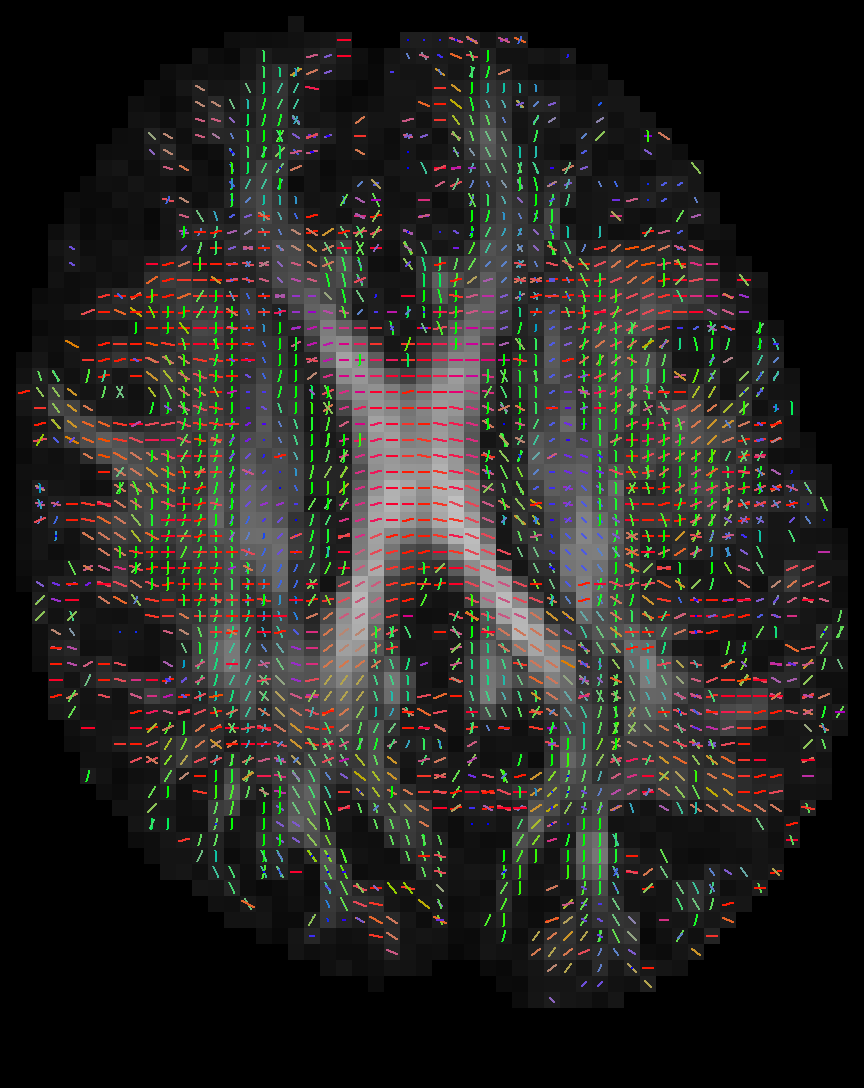
\includegraphics[scale=0.4]{figures/dsi_studio_result}
\par\end{centering}

\caption{Multiple crossings of a real human data set using Quantitative Anisotropy.
The first component of QA ($QA_{0}$) is also shown in the background.}


\label{Flo:QA_directions}
\end{figure}



\subsubsection{Robustness of QA}

GQI was shown to have comparable accuracy to other well established
q-space methods when it comes to resolving crossing fibres. In addition,
this is achievable with as few as $102$ points on a grid sampling
scheme, bringing the total acquisition time down to a clinically acceptable
level. Another advantage of GQI is that it is also applicable to a
shell sampling scheme. Despite their successes in tractography applications,
q-space techniques have until now failed to produce scalar metrics
that could replace the ones derived from the diffusion tensor model
(e.g. mean diffusivity, MD, and fractional anisotropy, FA) in terms
of their multi-subject comparability and specificity to pathology.
The data acquired with a grid sampling scheme can still be used to
estimate a diffusion tensor and respective scalar parameters, but
the effects of the high b-values required for q-space imaging ($>2,000s/mm^{2}$)
in the accuracy of the resulting DTI parameters has not been well
characterized. The authors of GQI have also proposed a new scalar
metric called quantitative anisotropy (QA) which was described in
the previous sections, but its properties have not been compared to
those of FA. In this section we will compare the estimated values
of MD, FA and $QA_{0}$ (first component of QA) obtained with grid
and shell sampling schemes, in terms of their precision and ability
to differentiate between different brain fibre populations.

%
\begin{figure}
[th!]

\begin{centering}
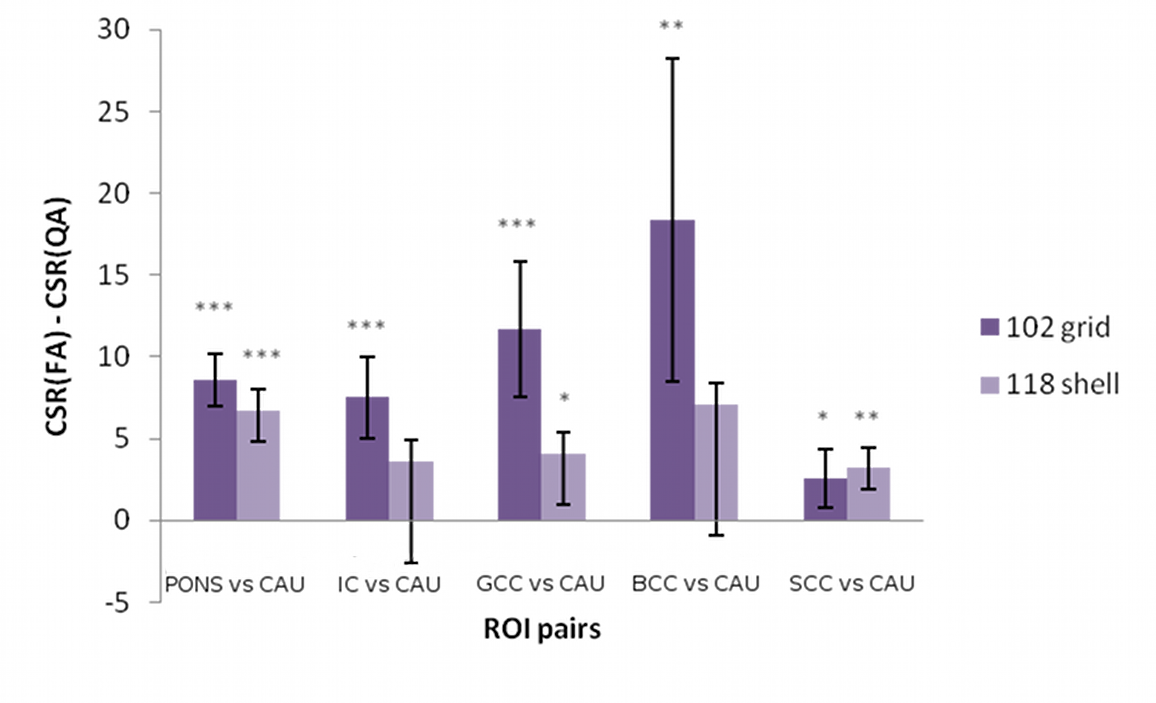
\includegraphics[scale=1.3]{figures/MartaISMRM2}
\par\end{centering}

\caption{Sample results of the paired t-tests comparing CSR (FA) and CSR ($QA_{0}$)}


\label{Flo:CSR_t-test}
\end{figure}


Twelve healthy volunteers aged between $18$ and $40$ were scanned
on a 3T scanner (TIM Trio, Siemens), using Siemens advanced diffusion
work-in-progress sequence, and STEAM \cite{merboldt1992diffusion,MAB04}
as the diffusion preparation method. The field of view was $240\times240\,\textrm{mm}^{2}$,
matrix size $96\times96$, and slice thickness $2.5\,\textrm{mm}$
(no gap). $55$ slices were acquired to achieve full brain coverage,
and the voxel resolution was $2.5\times2.5\times2.5\,\textrm{mm}^{3}$.
Two sampling schemes were considered: a 102-point grid acquisition
with a maximum b-value of $4,000\,\textrm{s}/\textrm{mm}^{2}$, and
a single shell acquisition using $118$ non-collinear gradient directions
and a b-value of $1,000\,\textrm{s}/\textrm{mm}^{2}$ \cite{correia_garyfallidis2011}.
The two acquisition schemes were matched for total acquisition time
in (14 min 37~s), voxel resolution, and bandwidth. FA, MD and $QA_{0}$
maps were then generated for each acquisition scheme and for the $12$
volunteers using $\texttt{DIPY}$ \cite{garyfallidis2011dipy}. All
the FA datasets were non-linearly registered into MNI space using
FSL tools, and the same transformation parameters were applied to
MD and $QA_{0}$ maps . Fourteen ROIs of different brain regions were
drawn in MNI space: Putamen (left and right), Caudate (left and right),
Thalamus (left and right), Para-sagittal white matter (left and right),
Pons, Internal Capsule (left and right), and Genu, Body and Splenium
of the Corpus Callosum. Small cubic ROIs were also constructed by
finding the centroid of each anatomical ROI and using it as the centre
for a $3\times3\times3\,\mathrm{mm}^{3}$ ROI. For each ROI we calculated
the mean value for each metric, and the spatial coefficient of variation
(CV) within the ROI (see Eq.~\ref{eq:CV_roi}). \begin{eqnarray}
CV_{ROI} & = & \frac{\sigma_{x}}{<x>}=\frac{N_{voxels}\sqrt{\sum_{x_{i}\in ROI}(x_{i}-<x>)^{2}}}{\sqrt{N_{voxels}-1}\sum_{x_{i}\in ROI}x_{i}}\label{eq:CV_roi}\end{eqnarray}


The coefficient of variation of each ROI mean across subjects was
also calculated, as a measure of each metric\textquoteright{}s comparability
between subjects. The contrast-to-scatter ratio (CSR) (calculated
for FA in Eq.~\ref{eq:CSR_FA}) is a good measure of a metric\textquoteright{}s
ability to differentiate between different brain fibre populations
\cite{correia_garyfallidis2011}. \begin{eqnarray}
CSR(FA) & = & \frac{mean(FA)_{ROI_{1}}-mean(FA)_{ROI_{2}}}{\sqrt{var(FA)_{ROI_{1}}+var(FA)_{ROI_{2}}}}\label{eq:CSR_FA}\end{eqnarray}


Combining the left and right versions of each ROI, we have $9$ ROIs
of different brain populations, which can be used to define $36$
pairs of ROIs, and the CSR of all metrics was calculated for each
of these pairs. Paired t-tests were then conducted to compare the
performance of each metric with the two acquisition schemes, and also
to compare FA and $QA_{0}$ directly for each acquisition scheme. 

%
\begin{figure}
[th!]

\begin{centering}
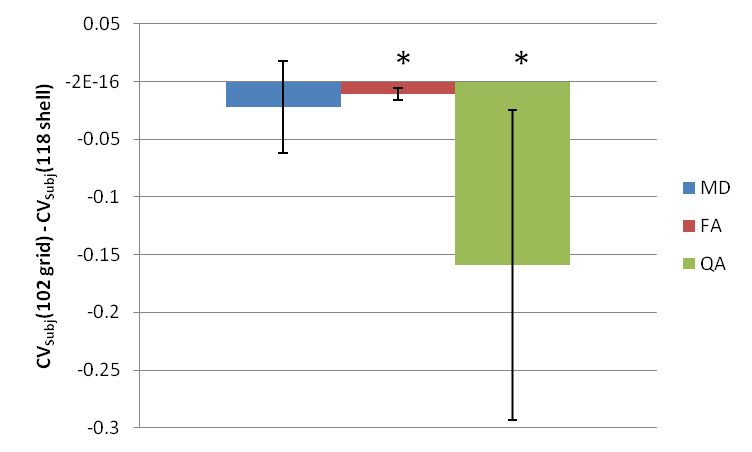
\includegraphics{figures/MartaISMRM1}
\par\end{centering}

\caption{Results of the paired t-test comparing the CVs across subjects for
MD, FA and QA0.}


\label{Flo:t-test_QA0}
\end{figure}


The $102$ grid sampling scheme produces significantly higher mean
FA and $QA_{0}$ values than the ones obtained with the $118$ shell
scheme, while the opposite was observed for MD. The CSR results for
FA and QA0 were not significantly different between the two acquisition
schemes, but the $102$ grid scheme produces significantly higher
CSRs for MD for 26/36 ROI pairs (Fig.~\ref{Flo:CSR_t-test}). For
MD, no significant different was found for the CV across subjects,
but for FA and QA0 the 102 scheme produced results more comparable
across the different volunteers (Fig.~\ref{Flo:t-test_QA0}). For
FA and MD the $102$ scheme showed lower CV within ROIs, especially
for white matter, but no difference was found for $QA_{0}$. When
comparing FA and $QA_{0}$ directly, our results show that FA produces
higher CSRs than QA0 for $23/36$ ROI pairs for the $102$ grid sampling,
and for $19/36$ ROI pairs for the $118$ scheme. FA also shows lower
variation across subjects for both acquisition schemes. Finally, FA
showes lower CVs within white matter ROIs, while $QA_{0}$ shows less
variability for grey matter. The results described and shown above
were obtained with the cubic ROIs, but do not differ significantly
when the same analysis was applied to larger anatomical ROIs.

Our results indicate that the MD and FA maps generated from a grid
sampling scheme designed for GQI are still suitable for analysis,
since they do not show poorer performance when compared to a single
shell and low b-value acquisition. In fact, the overall results suggest
that the $102$ grid sampling produces slightly more robust results
than the $118$ shell acquisition. A previous study \cite{correia2009looking}
has shown that metrics such as MD and FA benefit from the use of multiple
b-values, which could explain the better performance of the $102$
grid scheme.


\subsection{Discussion and Conclusion}

Non-parametric methods have the advantage of representing the signal
with minimum number of assumptions and without needing any fitting.
For many years there has been a trend in science to prefer model-based
rather than model free (non-parametric) methods. This is perhaps because
model-based can be easier to describe, and allow the use of popular
Bayesian approaches more readily. However, there are some crucial
issues with fitting: (a) Usually the interesting models have many
parameters and that makes fitting very slow. (b) Commonly non-linear
fitting is needed and accurate fitting is not trivial. (c) Often the
model does not represent precisely the complexity of the real problem.
(d) The more complex the model, the more difficult to fit \cite{rice2006mathematical},
\cite{lee1997bayesian},\cite{montgomery2001introduction}. 

Non-parametric methods avoid fitting model parameters and that gives
them a big advantage. The focus of this chapter was on introducing
and developing new non-parametric methods (EIT) or comparing and extending
existing ones (GQI2). We showed that a simple, fast and comprehensive
transform exists that we call the Equatorial Inversion Transform (EIT).
With this transform we showed that we can represent accurately the
directional information of the diffusion signal. Furthermore, we showed
that there are many different functions ($F$ and $O$ see Eq.~\ref{eq:ODF_EIT},
\ref{eq:eit_operator}, \ref{eq:eit_radial_weighting}) which can
be used in order to create spherical density functions and use these
to find the primary fibre directions. With a correct choose of $F$
and $O$ we can create theoretically the same ODF as the real ODF
(DSI ODF). This can be done using EITL which is a type of EIT. Nonetheless,
other density functions can be created that can identify the leading
fibre directions without being real ODFs but they are still different
types of spherical densities. EITL2 and EITS are examples of this
last case. 

The EIT concept opens new doors for the investigation of dMRI where
many new functionals can be invented in the future that emphasise
different properties of the signal. We have already illustrated and
measured that EIT has the best performance with simulations against
the state-of-the-art methods like DSI and GQI and that empirically,
EIT gives as good results with real data sets.

The EIT finds the ODF directly without creating the diffusion propagator.
If for some purpose the diffusion propagator is still required, then
DSI or DPI \cite{descoteaux2010multiple} are favourable. It could
be interesting in the future to try and recover the propagator using
ideas from the EIT. However, nearly always the propagator is not needed
for the analysis. Furthermore, comparing 4D densities like the propagator
is a non-trivial problem, also storing the propagator for every voxel
is very inefficient.

We discussed that GQI can be used for creating Quantitative Anisotropy
(QA). We observed that QA acts like a differential operator. It bears
some similarities with FA as it is maximum on anisotropic and $0$
on isotropic voxels. QA assumes that a substantial isotropic part
can always be removed from the ODF and that makes it more favourable
for spherical functions like those of GQI and EITS. This is in contrast
to sharper densities like those of DSI and GQI2 where QA is not as
useful because the minimum value of these densities will be usually
near $0$. 

GQI needs a manually set parameter; the diffusion sampling length
and in contrast the EIT is fully automatic i.e. we always just used
the few default parameters for all experiments. The diffusion sampling
length can be slightly different from experiment to experiment. The
asset of GQI and GQI2 (which was presented together with GQI but not
investigated until today) is that they are fast to compute and have
simple analytical solutions. GQI2 seems robust and smooth and it has
good performance both with simulations and real data. 

It is important to stress that there are similarities between all
these methods; DSI is similar to EITL, GQI to EITS, GQI2 to EITL2.
In addition, we showed that we can denoise the signal using a Gaussian
Spherical Angular method which operates on spherical densities and
has a single parameter which is similar to the variance.

Finally, we showed that the first component of QA (highest QA value)
can be used for subject comparisons in a similar way to FA. We also
showed that NPA could replace FA if we want to calculate anisotropy
in a completely geometric way. 

The source code for all the methods analyzed in this chapter is available
at $\texttt{dipy.org}$ under module $\texttt{dipy.reconst}$.

\selectlanguage{british}%

